\PassOptionsToPackage{hyperref}{hyperindex}
\documentclass[nda]{trkalray}
%\documentclass[colorlinks]{trkalray}
\usepackage{xspace}

%\PassOptionsToPackage{table}{xcolor}
\usepackage{graphicx}
\graphicspath{{images/}}

\IfFileExists{slashbox.sty}{\usepackage{slashbox}}{\usepackage{diagbox}}
%\usepackage{lscape}  % for landscape operation codes
\usepackage{pdflscape}  % for landscape operation codes + rotate pages in pdf (but still ok to print)
%\usepackage{srcltx}  % source reversal
\usepackage{colortbl}% for colors in tables
\usepackage{hhline}  % for lines in tables
\usepackage{multirow}
\usepackage{bitfields}

\usepackage{multicol}
\usepackage{tabularx}

%\usepackage[hyperindex]{hyperref}
\usepackage{makeidx}
\makeindex
%\newindex{default}{idx}{ind}{Instruction index}

\ifx\onlyinput\undefined\else
  \let\oldinput=\input
  \def\input#1{{
    \def\x{#1}
    \ifx\x\onlyinput\oldinput{#1}
    \fi
    }}
  \overfullrule=5pt
\fi

\newcommand{\KalrayK}{{Kalray kv4}\space}

\setcounter{tocdepth}{3}

\version{KETD-62}{W25}{2019}

\title{Kalray kv4 V1 VLIW Core Architecture Manual}
\titlelabel{KalrayKv4VLIWCoreArchitectureManual}

\docowner{Beno\^{\i}t Dupont de Dinechin}{benoit.dinechin@kalray.eu}

\author{%
Kalray S.A.\autref{1}
}
\institute{%
\autlabel{1} \email{info@kalray.eu},
Kalray S.A.
}

\abstract{Instruction Set Architecture and Micro-Architecture
of the \KalrayK core.}

\keywords{%
VLIW, DSP
}

\newcommand{\clusterdoc}{\emph{\MPPA{} Cluster Architecture}\space}

\begin{document}
\maketitle

\tableofcontents

\newpage
\section{Core Architecture}

\subsection{VLIW Architecture}

The \KalrayK core implements a 64-bit 8-issue Very Long Instruction
Word (VLIW) architecture with a 8-stage instruction pipeline. Groups of
instructions that issue together are identified and encoded by the assembler into
\emph{instruction bundles} (or ``bundles''). Inside a bundle, the source registers of all instructions are read before any target register is written. This key feature of VLIW execution enables to swap two registers by bundling two copy instructions that target each other source register. In also enables to expose wider SIMD instructions that what the ISA proposes by bundling them.

Compared to traditional VLIW architectures, whether Fisher-style or EPIC-style, the distinguishing features of the \KalrayK architecture are:
\begin{itemize}
    \item No need for inserting NOP instructions to complete bundles (horizontal NOPs) or to satisfy register dependences (vertical NOPs).
    \item Individual instructions are 32-, 64- or 96-bit wide in order to inline the 32-bit or 64-bit immediate constant operands.
    \item The core appears as a in-order superscalar to the compiler, as any parallel instruction group identified by instruction scheduling can be encoded in a bundle.
    \item Support of predication and masking for any non-control instruction without the cost and complexity of a fully predicated ISA by bundling dedicated control unit instructions.
\end{itemize}

The \KalrayK core architecture has 64$\times$64-bit general-purpose registers (GPRs) that
contain boolean, integer, address, fixed-point and floating-point data types. The core supports the corresponding arithmetic instructions and also their SIMD versions on 128-bit data held into register pairs.
The \KalrayK core architecture is byte-addressable little endian. The architecture is also
a bit-little endian, meaning that bit 0 of any data is always the least significant bit
(little endian), and is shown at the rightmost position in figures.

The \KalrayK core architecture supports an optional coprocessor extension (historically called TCA) which is tightly integrated into the instruction pipeline. This coprocessor extension hosts a 32$\times$512-bit register file is aiming at accelerating compute intensive applications using 512-bit SIMD arithmetic. The coprocessor extension itself can be further connected to external compute resources to expand the core capabilities.

\subsection{Data Types and Representations}

The \KalrayK core instruction set architecture (ISA) efficiently supports 8-bit,
16-bit, 32-bit, 64-bit, and 128-bit scalar types, and also 8-bit, 16-bit, 32-bit or 64-bit data
types packed into 128-bit containers. The non-packed data types are interpreted as
signed integers, unsigned integers, and IEEE~764 binary floating-point numbers.

\subsubsection{Signed Integers}

An integer is expressed as a binary number of 2's complement and is 8-, 16-,
32-, 64-bit, or 128-bit long. Regardless of its length, the bit 0 of an integer
is always the least significant bit. Because 2's complement is used, the most
significant bit is used as a sign bit.

\begin{center}
\begin{tabular}{|c|c|} \hline
{Data Length} & {Value Range} \\ \hline
{8 bits} & $-2^7$ to $+2^7 - 1$ \\
{16 bits} & $-2^{15}$ to $+2^{15} - 1$ \\
{32 bits} & $-2^{31}$ to $+2^{31} - 1$ \\
{64 bits} & $-2^{63}$ to $+2^{63} - 1$ \\
{128 bits} & $-2^{127}$ to $+2^{127} - 1$ \\ \hline
\end{tabular}
\end{center}

\subsubsection{Unsigned Integers}

An unsigned integer is a binary number whose most significant bit has a positive
weight and is 8-bit, 16-bit, 32-bit, 64-bit, or 128-bit long.

\begin{center}
\begin{tabular}{|c|c|} \hline
{Data Length} & {Value Range} \\ \hline
{8 bits} & $0$ to $+2^8 - 1$ \\
{16 bits} & $0$ to $+2^{16} - 1$ \\
{32 bits} & $0$ to $+2^{32} - 1$ \\
{64 bits} & $0$ to $+2^{64} - 1$ \\
{128 bits} & $0$ to $+2^{128} - 1$ \\ \hline
\end{tabular}
\end{center}

\subsubsection{Floating-Point Numbers}

The \KalrayK core represents floating-point numbers in little-endian binary
format, according to the IEEE754~2008 standard.

For 16-bit binary floating-point numbers, the representation is as follows:

\bitfields{ 1/s, 5/exponent, 10/fraction}

For 32-bit binary floating-point numbers, the representation is as follows:

\bitfields{ 1/s, 8/exponent, 23/fraction}

For 64-bit binary floating-point numbers, the representation is as follows:

\bitfields{ 1/s, 11/exponent, 20/fraction, 32/fraction}

\subsubsection{Load and Store Instructions}

Load and stores transfer data between between the general purpose registers of the core and addressable memory. Data transfers width is any of 8, 16, 32, 64, 128, or 256 bits:
\begin{itemize}

\item Loading 8-bit, 16-bit and 32-bit from memory produces a 64-bit word by either sign-extending or zero-extending the loaded value.

\item When loading 64-bit data, they are directly stored into the target
  register.

\item When loading 128-bit data, they are directly stored into the target
 register pair ($R_{i}$ and $R_{i+1}$, with $i$ even).

\item When loading 256-bit data, they are directly stored into the target
 register quadruple ($R_{i}$ to $R_{i+3}$, with $i$ multiple of 4).

\end{itemize}


\subsection{VLIW Instruction Bundles}

\subsubsection{Instruction Bundle Composition}

The \KalrayK instruction bundle is composed of 32-bit instruction syllables. Instruction syllables in a bundle encode up to two BCU (Branch \& Control Unit) instructions, two ALU (Arithmetic \& Logic) instructions, two LSU (Load-Store Unit) instructions, two EXT (coprocessor Extension) instructions, and up to eight IMMX (Immediate Extension).
For each syllable: \begin{itemize}
\item Bit 31 is the Parallel bit: 0 if syllable is last in the bundle, else 1.
\item Bits 30 and 29 encode the Steering: 0 for BCU; 1 for LSU; 2 for ALU; and 3 for EXT.
\item Immediate extension (IMMX) syllables have Steering 0 and provide 27 bits of payload.
\item An IMMX  syllable specifies its target with a 2-bit Tag encoded in bits 28 and 27.
\end{itemize}

The \KalrayK architecture provides issue slots called BCU0, BCU1, ALU0, ALU1, LSU0, LSU1, EXT0, EXT1 that correspond to execution units (EXUs).
\begin{itemize}
\item The IMMX syllable Tag specifies its target issue slot as: 0 for ALU0; 1 for ALU1, 2 for LSU0; 3 for LSU1.
\item One or two IMMX syllables may apply to any of the ALU or LSU instructions.
\item A BCU instruction may also benefit from a branch offset extension by positioning a syllable with Steering = 0 and Tag = 0 next to it.
\item Instructions executed on the EXT EXUs may not receive an immediate extension.
\item The maximum number of syllables in an instruction bundle is 18, but the number accepted in a valid bundle is set to 16.
\end{itemize}

Instructions that are PC-relative are based on the PC of their first syllable in the bundle.

\subsubsection{Operand Immediate Extensions}

The core subset of 64-bit integer instructions and load/store instructions may encode a signed 10-bit immediate operand. With one IMMX syllable, a 37-bit signed immediate operand is available. With two IMMX syllables, a 64-bit immediate operand is available. Moreover, instructions called MAKE may encode a 16-bit signed immediate in a single syllable:

\begin{center}
\begin{tabular}{|l|l|l|} \hline
Instruction Type & Immediate Constant & Instruction Size \\ \hline
MAKE & 16 bits signed & 32 bits \\
MAKE & 37 bits signed & 64 bits \\
MAKE & 64 bits & 96 bits \\
ALU, LSU & 10 bits signed & 32 bits \\
ALU, LSU & 37 bits signed & 64 bits \\
ALU, LSU & 64 bits & 96 bits \\ \hline
ALU & 32 bits signed & 64 bits \\
SIMD & 32-bit splatted & 64 bits \\
\hline \end{tabular}
\end{center}

In this table, the two last rows correspond to the so-called "magic immediate" extensions. In this case, the base instruction does not have a 10-bit signed immediate operand that could be extended. Rather, its source operands are GPRs specified by a 6-bit field. When an IMMX syllable targets such an instruction, the 6-bit register specifier is interpreted a one 'splat' bit and 5 payload bits. The 5 payload bits and the IMMX 27-bit payload provide 32 bits. These 32 bits are either sign-extended, or the 32 bits are replicated to the operand width. The latter is useful to provide immediate operands to SIMD instructions with up to 32-bit wide lanes.

\subsubsection{Instruction Bundle Binary Layout}

Instructions in a bundle are dispatched to the \KalrayK issue slots in the order BCU0, BCU1, ALU0, ALU1, LSU0, LSU1, EXT0, EXT1. So the first syllable of any instruction must follow this order in the bundle binary layout. The immediate extension syllables (Steering = 0) for ALU and LSU instructions must appear last in the bundle with the least significant bits of payload first in case of instructions with two IMMX syllables. In case of a BCU instruction with extended offset, its IMMX appears as the second syllable (the first being the branch instruction).

Moreover, instructions dispatch starts by the EXUs that have the most capabilities: \begin{itemize}
\item BCU0 may execute all BCU instructions, while BCU1 only accepts BCU instructions that may dual issue.
\item ALU0 may execute all ALU FULL instructions and ALU1 may execute all ALU LITE instructions. LSU0 and LSU1 may execute the ALU TINY instructions.
\item LSU0 may execute all the LSU instructions, while LSU1 only accepts the load and DTOUCHL instructions.
\item EXT0 may execute the COMP instructions, and EXT1 the MISC instructions.
\end{itemize}

\smallskip
%{\color{red}Please refer to Section~\ref{sec:encoding} for the details of instruction bundle encoding.}

\subsubsection{Instruction Bundles in Assembly Language}

At the assembly language level, instructions may appear in any order (except for branch instruction that are ordered) and the immediate operand extensions are not apparent. These extensions are inferred from the number of bits required to encode the immediate values.

Each assembler instruction is separated from the next one either by an end of line or by a `\texttt{;}' character. The end of the bundle is marked by a `\texttt{;;}' alone in its line. Like with most assembly languages, a single `\texttt{\#}' character introduces a comment that extends until the end of line.

At the assembly language level, the control instructions that drive instruction predication or masking of other (non-control) instructions in the bundle do not appear explicitly. Rather, the assembler collects the prefix syntax of the predicated or masked instructions, and consolidate them as separate control unit instructions in the bundle binary encoding.

\section{Core Implementation}

\subsection{Datapath Organization}

\subsubsection{Execution Units and Register Files}

The \KalrayK core includes two main arithmetic, logic and floating-point units that include
multiply-accumulate instructions (ALUs), two load/store units (LSUs) and two branch/control unit (BCUs).
These six execution units are primarily connected through the GPR register file, that supports
reading up to eleven 64-bit registers plus two 256-bit register quadruples, and writing up to
one 64-bit register, two 128-bit register pairs and two 256-bit register quadruples per clock
cycle. The six execution units also share system function registers (SFRs) for program control
and compute status (Figure~\ref{fig:dolomites-vliwcore}).


\begin{figure}
\centering
  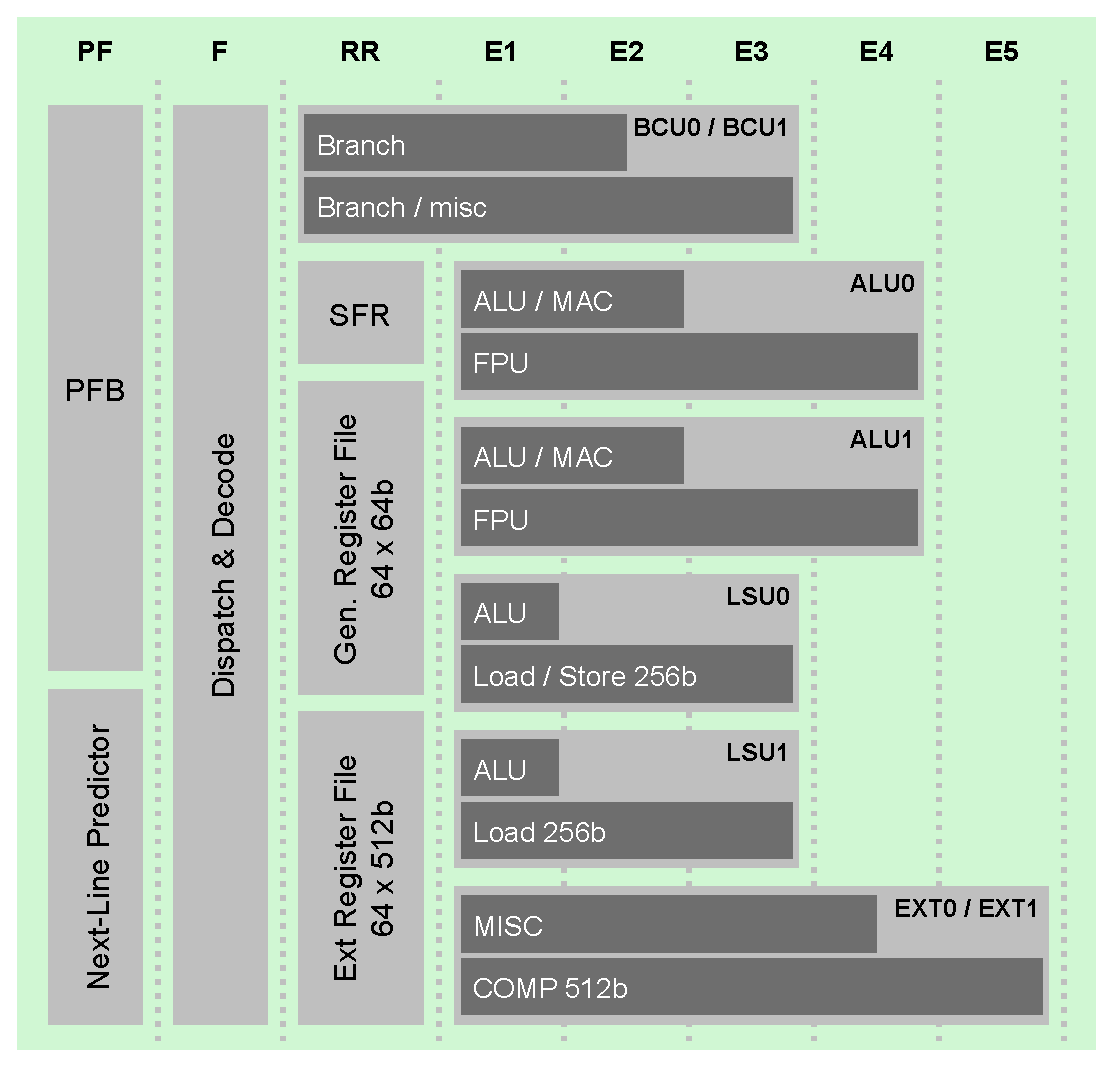
\includegraphics[width=.5\textwidth]{dolomites-vliwcore}
\caption{\KalrayK VLIW core block diagram.}
\label{fig:dolomites-vliwcore}
\end{figure}


\subsubsection{Instruction Pipeline Stages}

The instruction pipeline is composed of a Prefetch (PF) stage, a Fetch stage (F) and a Register
Read (RR) stage, followed by five execution stages: E1, E2, E3, E4, and E5 (coprocessor extension).
All executions begin in E1, with the exception of branches that are computed and taken as soon as
resolved by the branch predictor at ID or RR stage. Most operands are read or bypassed for 
execution at the end of RR. This pipeline allows arithmetic and load/store
instructions to execute for up to four cycles if needed. The results of instructions that
complete earlier than E4 are made available for bypassing as operands to subsequent instructions.

The instruction pipeline of the \KalrayK core is interlocked, i.e., run-time
stalls occur whenever an instruction tries to access a register that is not
data-ready.


\subsubsection{Prefetch Buffer (PFB)}

The Prefetch Buffer (PFB) is in charge of fetching instruction bundles and
preparing instructions for dispatch to the execution units.
The PFB manages 4 lines of 8$\times$32-bit and
receives blocks of 8$\times$32-bit from the instruction cache every clock cycle,
assuming that these blocks are in the instruction cache (fetch hit) and do not
cross a level-1 cache line boundary (64-byte).

The PFB attempts to fetch ahead in order to keep its 4 lines of 8$\times$32-bit
full. When a branch is taken, the PFB is flushed and a new fetch starts from the
target address. After a branch, the PFB takes one cycle to fetch the next bundle
from the cache. Branching to a bundle that is split over two cache lines
requires two cycles to fetch the bundle.

The PFB also provides 0-cycle overhead hardware loop support, allowing to
automatically jump from the end to the beginning of a hardware loop without
branch penalty.

\subsubsection{Branch and Control Unit (BCU)}

The \KalrayK core has two branch and control units (BCUs).
These units support PC-relative and indirect branches or calls. One branch unit also supports
hardware looping, also known as zero overhead loops.
Due to instruction pipelining, all taken branches (not including hardware looping) involve
run-time stalls: one cycle for unconditional direct branches and two cycles for
conditional and indirect branches. Not taken conditional branches involve no
stalls. Branch stalls are not visible at the architecture level, that is, there
are no delayed branches.
Up to two conditional branches, or one conditional branch and one unconditional branch (including function call/return), or one branch with extended offset, can be bundled with non-control instructions.
Branches within a bundle are ordered, so the first branch resolved as taken effectively branches ignoring the second one, even if the latter resolves as taken.

The BCU also supports predication and masking of other instructions in the bundle:
\begin{itemize}
    \item Predication allows a subset of instructions in the bundle to be conditionally disabled, depending on a predicate evaluated in one of the two BCUs. Predication is achieved by executing a GUARD instruction, which evaluates the same condition as the conditional branch instruction CB, but whose last operand is a 8-bit mask where each bit specifies the execution unit (ALU0, ALU1, LSU0, LSU1, EXT0, EXT1, ...) to be predicated.

    \item Similarly, the output of data processing instructions can be masked at the granularity of a 8-bit, 16-bit, 32-bit, 64-bit SIMD lane by executing a BLEND instruction, which specifies its target execution units with the same 8-bit mask as GUARD. The BLEND instruction reads a source operand where each bit corresponds to a SIMD lane, with the byte size of the lane provided by a modifier, and the masked instructions only write the active lanes.
\end{itemize}

In case of clusters composed of several processing elements (PE), each \KalrayK PE core is connected to its direct predecessor and successor by wires that transport events for direct
synchronization. The BCUs executes all instructions related to waiting and signaling events.

\smallskip 
%{\color{red}See Section~\ref{sec:BCU-instructions} for BCU instructions.}

\subsubsection{Arithmetic and Logic Units (ALUs)}

The \KalrayK core has two main arithmetic and logic units (ALU0 and ALU1). These units operate on both integer and floating-point values.

\paragraph{ALU Integer Operations}
Each arithmetic and logic unit (ALU) is capable of executing one instruction per cycle on 64-bit integers or on 128-bit SIMD integer data. Integer signed, unsigned, and signed saturated instructions are available on each ALU. The results of the ALUs are 64-bit or 128-bit wide and can be used as operands of the next instruction bundle (one clockycle latency), except for multiplication- and division-related instructions. In addition, the ALUs are capable of executing specific instructions such as building immediate values up to 64 bits (MAKE), adding constants to the instruction PC (PCREL), inserting/extracting bit-fields from 64-bit words, and moving data from/to the coprocessor extension.

\smallskip 
%{\color{red}See Section~\ref{sec:ALU-instructions} for integer instructions.}

\paragraph{ALU Floating-Point Operations}

The \KalrayK core ALUs perform floating-point operations on 16-bit (binary16 or FP16), 32-bit (binary32 or FP32) and 64-bit (binary64 or FP64) IEEE~754 floating-point formats and include addition, multiplication, multiply-add, comparisons and conversion from/to integer formats. All IEEE~754 standard rounding modes are supported, with the addition of the round-to-odd mode. All FPU operations correctly operate on the subnormal values. The only deviation from the IEEE~754 standard is that a canonical NaN is produced if any input or the result on an operation is a NaN.

The \KalrayK core ALUs include a dual multiply-add unit (FMA) in
single precision and a multiply-add unit in double precision. All floating-point
instructions operate in conformance with the IEEE~754-2008 standard for binary
floating-point numbers, including sub-normals and four rounding modes. Correctly
rounded division and square root instructions are available by executing
Newton-Raphson iterations on values provided by seed generators for the 32-bit
and 64-bit floating-point $\frac{1}{x}$ and $\frac{1}{\sqrt{x}}$.

\smallskip
%{\color{red}See Section~\ref{sec:FPU-instructions} for Floating-point instructions.}

\subsubsection{Load/Store Units (LSU)}

The \KalrayK core has a two load/store units (LSUs); they are fully pipelined with a latency of three cycles in the data cache. These units can take up to three operands (two 64-bits operands for the effective base+offset address computation, and one up to 256-bits for the stored data).
At every clock cycle, the core is able to do two loads of 256, 128 or 64 bits to registers
(simple, double or quadruple) or one load and one store of 256, 128 or 64 bits to/from registers
(simple, double or quadruple). When reading less than 64 bits from memory, load instructions zero-extend or sign-extend the memory datum to the 64 bits of the destination register.
Loads and stores are also available to the coprocessor EXT with data widths of 256 bits. \medskip

The LSU also supports atomic memory operations in various data sizes:

\begin{tabular}{|c|c|c|} \hline
{basic operation} & {logic operations} & {supported sizes} \\ \hline
load  & add, set, xor, clear, saturating decr & 1B, 2B, 4B, 8B \\
store & add, set, xor, clear & 1B, 2B, 4B, 8B \\
swap  & -                    & 1B, 2B, 4B, 8B \\
compare and swap (valued)  & - & 1B, 2B, 4B, 8B, 16B  \\
compare and swap (boolean) & - & 1B, 2B, 4B, 8B, 16B  \\ \hline
\end{tabular} \medskip

The \KalrayK core supports the following addressing modes for regular memory accesses:
\begin{itemize}
\item A base register plus a 10-bit signed, unscaled immediate constant.
\item A base register plus a 37-bit signed, unscaled immediate constant.
\item A base register plus a 64-bit signed, unscaled immediate constant.
\item A base register plus or minus an index register.
\end{itemize}

The \KalrayK core supports the following addressing modes for atomic memory accesses:
\begin{itemize}
\item A base register only.
\item A base register plus a 27-bit signed, unscaled immediate constant.
\end{itemize}

In non-device memory areas, the \KalrayK core supports memory accesses with
misaligned effective addresses for regular loads/stores.  Atomic instructions
and accesses to device memory areas must be aligned on the size of the accessed
object. If not, the \KalrayK core will take a DMISALIGN trap.

In order to speed up integer intensive applications, each LSU also includes a 64-bit
light ALU unit that execute a subset of the 64-bit arithmetic and logic instructions.
This light ALU can be used if the corresponding LSU is not used for memory access
instructions in the same bundle.

\smallskip
%{\color{red}See Section~\ref{sec:LSU-instructions} for LSU instructions.}


\subsubsection{Instruction Scheduling Constraints}

In addition to the bundle structure, which is defined at the architecture level, instruction scheduling is further constrained by micro-architecture resource and latency constraints. In particular, the Write-After-Read (WAR) dependence latency is zero, the Write-After-Write (WAW)
latency is one, and the Read-After-Write (RAW) dependence latency is strictly positive.

%{\color{red}\smallskip Please refer to Section~\ref{sec:constraints} for detailed instruction bundling constraints.}

The \KalrayK core scheduled resources abstract the hardware resources shared by instructions simultaneously issued on different execution units. These resources correspond to the register file access ports that are not dedicated to a particular execution unit (Figure~\ref{fig:regfile-kv4}): \begin{description}
\item[AUXR] LSU0 uses a 256-bit read port of the core registers at E1 to supply the stored values and execute read-modify-write atomic instructions.
\item[AUXW] Two 256-bit write ports of the core registers are used at E3, respectively, by LSU0 and LSU1 to receive the loaded values.
\item[MEMW] Ensures single issue of memory store and atomic instructions.
\item[SSFU] A 512-bit operand read port at RR of the MISC unit is shared with the SIMD SFU unit.
\item[ACCR] The 512-bit accumulator read port at E1 of the COMP unit is used by LSU0 to store extension register values (XSO instructions) and by the ALUs to get values from the extension registers (XMOVEF* instructions).
\item[OUTW] The 1024-bit output port at E2 of the MISC unit is used by the core to move values to the extension registers (XMOVET* instructions).
\end{description}

\begin{figure}
\centerline{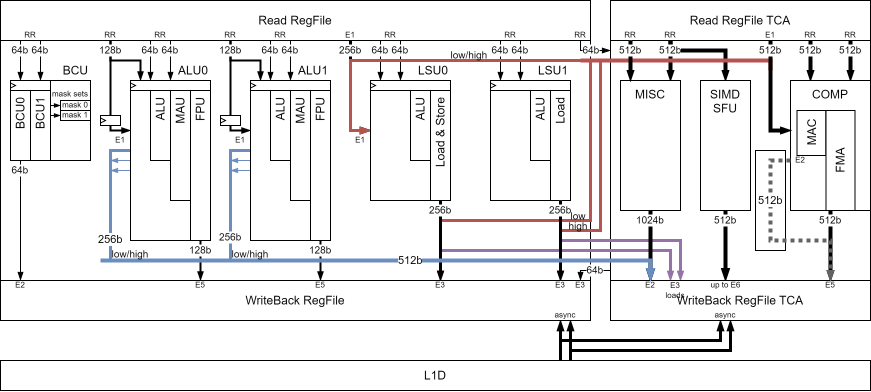
\includegraphics[width=1.25\columnwidth]{regfile-kv4}}
\caption{\KalrayK core register files accesses.}
\label{fig:regfile-kv4}
\end{figure}


\subsection{Memory Subsystem}


The \KalrayK core memory subsystem includes the following components: \begin{itemize}

\item Processor cache arbiter (PCA).
\item Instruction cache (IC).
\item Data cache (DC).

\end{itemize}

\subsubsection{Processor Cache Arbiter (PCA)}

The \KalrayK core features separate instruction and data caches that support,
respectively, the fetch of instructions and the load/store data accesses.
These two independent caches are connected to the outside memory system by a
round-robin arbiter: the PCA.

\subsubsection{Memory Management Unit (MMU)}

The \KalrayK core includes a memory management unit that performs address translation, ensures memory protection between processes and enforces memory caching and sharing policies. The MMU is described in detail in ~\ref{sec:memory-management-unit}

\subsubsection{Instruction Cache (IC)}

The instruction cache of the \KalrayK core receives fetch requests from the PFB
and returns groups of up to eight 32-bit syllables that will later be assembled
into bundles by the prefetch buffer. It has 32K bytes capacity, is 4-way set
associative with LRU (Least Recently Used) replacement policy and 64-byte
lines.

When the instruction words requested by the PFB are not in the cache, they are
fetched from the memory system (with a critical-word-first scheme) and stored
into the cache. During this time the core may stall, depending on the state of
the PFB. The requested syllables are then returned to the PFB.

To invalidate the instruction cache safely, the core must execute the IINVAL
instruction followed by the BARRIER instruction. This will invalidate the whole
instruction cache, and trigger a re-fetch that will flush the PFB and miss
in the invalidated instruction cache.

No hardware coherency mechanism exists with respect to the instruction cache.
Instruction cache lines need to be manually invalidated (using IINVAL*
instructions) to support, e.g. self-modifying code.


\smallskip
The instruction cache is globally disabled by clearing the ICE bit of the PS
register, see Section~\ref{sec:sfr}. The different instruction cache policies
(cache enable, cache bypass) are set by the Memory Management Unit, see
Section~\ref{sec:memory-management-unit}.

\subsubsection{Data Cache (DC)}

The data cache receives load/store/atomic requests from the LSUs and returns the
requested data to the core. The data cache has the following characteristics:
\begin{itemize}
\item write-through, no write-allocate
\item 64-byte line, 32K bytes capacity
\item 8-way set-associative, LRU eviction policy
\item supports hit under miss and hit under prefetch
\item supports 16 outstanding refills or prefetches
\item supports up to 32 primary and secondary misses (if they do not cross 32B boundaries)
\item banked memory organization interleaving cache sets onto 4 banks, to allow for simultaneous double LSU operation
\item way predictor based on the virtual addresses for power efficiency
\item nominal refill rate of 64 bytes per cycle

\end{itemize}

\begin{figure}
    \centering
    \includegraphics[width=.75\linewidth]{images/kv4_dcache_schematic.png}
    \caption{\KalrayK data cache block diagram.}
    \label{fig:enter-label}
\end{figure}

Store requests are directly sent to the memory, updating the cache on their way if
they hit. In case a cached store misses, no line allocation is done in the cache
and the store is simply posted to the memory.

If a store is aligned, uncached (by way of PS.DCE = 0, see Section~\ref{sec:sfr}) or MMU cache policy (see Section~\ref{sec:memory-management-unit}) and PS.USE = 0 , then the core will stop executing until it receives the answer fromthe memory system for that store. This allows to generate precise exceptions in case of memory bus error and thus ease the debug of (e.g.) code accessing devices.
In all other cases (misaligned or cached store or PS.USE = 1), stores are posted: the core does not wait for their answer and may continue executing, including submission of new LSU requests to the data cache; an erroneous response from the memory will trigger a DAME interrupt.

When data loaded by the core are not in the cache (primary load miss), they are
fetched from memory and eventually copied into the cache (line allocation). During this
time the core will stall if it tries to process an instruction that has a data
dependency on the loaded data, but can otherwise keep working with the cache 
(hit-under-miss is supported). Several loads can miss in a line that is under
refill ("secondary misses"). When the line data are handed to the cache by the memory
system, they are stored in a temporary "line buffer", and are used to respond to all
misses linked to that cache line (primary + secondary); then they are written to the cache memories for standard use on load hits.

As for the stores, an aligned uncached load with PS.USE = 0 will be considered as blocking.

If executing a load instruction with uncached modifier, or if PS.DCE = 0, or if
the address of a data access falls in a device or uncached memory area (be it
the default device memory map when the MMU is off or a device/uncached page with
MMU on), then the access is considered as uncached: it is simply forwarded to the
memory and, if applicable, the response is forwarded to the core, leaving the
cache contents unchanged.

\subsubsection{Memory Ordering}

The \KalrayK memory model is such as two accesses of the same nature
(cached or uncached) issued by the same core to the same memory location are
guaranteed to complete in program order. Accesses to different memory locations
are not guaranteed to complete in any particular order. A FENCE instruction can
be used to force all previously issued data memory accesses to complete before a new
data memory access can be issued by the core.  

Furthermore, misaligned write accesses crossing a 64-byte boundary may complete
in a non-atomic way, i.e. an other core reading at the same misaligned
address shortly after the write from the first core might see the update of
the bottom part but not that of the top part or conversely. Then again, the
execution of FENCE by a core guarantees that all the previous accesses of
this core (be they misaligned or not) have completed before it can emit new
data accesses.

Data L1 cache coherency is implemented using a directory in the shared memory
(SMEM) of the clusters grouping 16 \KalrayK cores. As a result, a store from
core 1 is guaranteed to be seen by a core 2 polling on the same SMEM address
with loads after some time (equal to the time taken by the store to reach the
memory plus a fixed number of cycles). If core 1 executes a FENCE after its
store, it is guaranteed that the store has been made visible to core 2 before
any new data access can be issued from core 1.

\newpage
\section{Core Accelerators}

The two \KalrayK core accelerators aim at providing an increased performance by processing in parallel large arrays of data. They are either full integrated in the core (EXT) and share its execution pipeline or driven by one or more core through control and data pipes (LCA).

\subsection{Tightly-Coupled Accelerator (TCA)}

The \KalrayK core may dispatch up to two instructions per bundle to a coprocessor
extension EXT implemented as a tightly coupled accelerator (TCA). This coprocessor includes a datapath and operators designed for 512-bit SIMD arithmetic and functions, including deep learning activation functions.
The coprocessor features 32$\times$512-bit registers, and associating them in pairs provide
1024-bit operands (Figure~\ref{fig:processor and accelerators}).

\smallskip 
%See Section~\ref{sec:EXT-instructions} for EXT instructions.

\begin{figure}
  \centering
  \includegraphics[width=.7\textwidth]{images/CORE-TCA-LCA.png}
  \caption{\KalrayK VLIW core and accelerators}
  \label{fig:processor and accelerators}
\end{figure}


The coprocessor extension EXT is part of the core pipeline and executes instruction from bundles fully synchronized to the scalar core. Dispatch and stall behavior matches the core scalar behavior.

The EXT has data interfaces to the LSUs, allowing direct load and store to the EXT registers from the data cache and main memory.
With the connection to both LSUs, the EXT can have 2 256-bit loads or one 256-bit load and one 256-bit store. Loads and stores access the upper or the lower part of the 512-bit EXT register file.

The EXT also has data interfaces to the general purpose register file allowing transfers of register content to and from the scalar pipeline.

The two execution units within the EXT process large vectors of 512-bit (up to 3 per unit) and produce 512-bit or 1024-bit results.

One unit is dedicated to compute operations: additions, multiplications, compare (on integer format from 8-bit to 64-bits and floating-point formats from 8-bits to 64-bits)
whereas the other handles data movements, simple functions (format adjustments) or special instructions.
The special instructions handle multi-cycle computing such as division and reverse square root.

\subsection{Loosely-Coupled Accelerator (LCA)}

The \KalrayK core coprocessor can be further connected to a Loosely-Coupled Accelerator (LCA)
to support large matrix processing. The LCA is a shared accelerator that executes instructions
issued by up to four cores.
The coprocessor acts as an interface for the instruction execution in the LCA by providing write and read channels as well as control commands to the LCA.

Execution in the LCA implies synchronization of the cores.
The LCA feature a set of input matrices of 1K-byte that can be used as a $32\times32$ 8-bit matrices, $32\times16$ 16-bit matrices or $32\times8$ 32-bit matrices.

The LCA executes matrix multiplications and accumulations (MMA) on 1KB matrices. Working on different formats, it performs the MMA on sizes 32$\times$32, 16$\times$32 and 8$\times$32.
It connects to the EXTs of 4 core. Its general structure is shown in figure~\ref{fig:LCA-diagram}.

\begin{figure}
  \centering
  \includegraphics[width=.5\textwidth]{images/LCA-diagram.png}
  \caption{\KalrayK LCA diagram}
  \label{fig:LCA-diagram}
\end{figure}

Matrices data are provided by data pipes from the EXT register files and stored in the LCA before processing. Matrix MMA results are returned to the EXT through a return path.
The 4 cores feed the LCA and ensure the bandwidth allows for sustained operation without cycle losses. Matrix MMA are shadowed so that no conflict arises from loading and processing.


\subsubsection{LCA supported sizes and formats}
The LCA supports 8-bit integer and 8-bit, 16-bit and 32-bit floating-point sources for the matrix operands. The accumulating matrix only support 32-bit (integer or floating-point, depending on source format).

\begin{center}
\begin{tabular}{|l|l|l|}
  \hline
  Format Name & Data Size & Format Detail \\
  \hline
  fp32 & 32-bit & Standard IEEE-754 binary 32 \\
  fp16 & 16-bit & Standard IEEE-754 binary 16 \\
  bf16 & 16-bit & Binary format with 1 sign bit, 8 exponent bits, 7 mantissa bits\\
  e5m2 & 8-bit & Binary format with 1 sign bit, 5 exponent bits, 2 mantissa bits\\
  e4m3 & 8-bit & Binary format with 1 sign bit, 4 exponent bits, 3 mantissa bits\\
  int8 & 8-bit & 8-bit signed integer \\
  uint8 & 8-bit & 8-bit unsigned integer \\
  \hline
\end{tabular}
\end{center}

\subsubsection{LCA integer MMA}
Integer Multiplication supports mixed int8 and uint8 matrices of 32$\times$32. The accelerator perform the multiplication of the two matrices and accumulate the result in a 32-bit integer array or 32$\times$32.

\subsubsection{LCA Floating-Point MMA}
\paragraph{8-bit float input types:} The accelerator multiplies two 32$\times$32 matrices and accumulate the result in a 32-bit floating-point array of 32$\times$32. Mixed 8-bit formats are supported.
\paragraph{16-bit float input types:} The accelerator multiplies one 32$\times$16 matrix by a 16$\times$32 matrix and accumulate the result in a 32-bit floating-point array of 32$\times$32.
\paragraph{32-bit float input types:} The accelerator multiplies one 32$\times$4 matrix by a 4$\times$32 matrix and accumulate the result in a 32-bit floating-point array of 32$\times$32.

\subsubsection{Data Streams}
Loading each matrix involves formatting and transposing according to the load attributes.
Input data streams come from each core. 512 bits can be transferred each cycle from each EXT to the target data matrices.
Specific core instructions initiate each unit transfer to the LCA.
Output data streams go to each core. 512 bits can transferred each cycle to each EXT. Specific core instructions load from the result pipeline to the EXT.

\subsubsection{Matrix computation}
Matrix multiplication is initiated by a core instruction from each core. Cores must be synchronized as the multiplication only starts when all 4 sources have provided data and validated the execution. It is up to the software to ensure that the core execute code compatible with this synchronization requirement.

\subsubsection{Types of operation}
Multiplication can use any matrix as source. The accumulation is optional and the previous accumulator is discarded when the accumulation is not required.
Accumulating across formats (integer/floating-point) is not allowed.

\subsection{Micro architecture of matrix multiplication}
The matrix multiplication uses individual dot-product operators that operate on two 32-byte vectors. A full matrix multiplication requires 1024 dot operations. For implementation reasons and to align with data bandwidth, only 1024/N operators are implemented. The full multiplication takes N cycles to complete.
Each dot-product operator processes the two 32-byte vectors according to the configured format, i.e. 32 8-bit integer per vector, 32 8-bit floats per vector, 16 16-bit floats per vector or 4 32-bit floats per vector.
As operators are re-used for N cycles, N accumulators are implemented per operator to maintain a total of 1024 accumulation values (a full accumulation matrix).
The format of the accumulators is an internal expanded format allowing an area/precision trade-off across all multiplication types.

\begin{figure}
\centering
  \includegraphics[width=1.0\textwidth]{images/LCA-matrix-multiplication.png}
\caption{\KalrayK LCA matrix multiplication}
\label{fig:LCA-matrix-multiplication}
\end{figure}


\subsubsection{Matrix storage}
There are 4 matrices available as MMA sources. Two are used for multiplication while the two others receive data from the cores.
Transposition is available for each matrix and each format, leading to 4 different configurations
\begin{itemize}
  \item Non transposed: all 32$\times$32, 32$\times$16, 32$\times$8 matrices overlap
  \item 8-bit transpose: transpose the 32$\times$32 matrix
  \item 16-bit transpose: transpose the 32$\times$16 matrix
  \item 32-bit transpose: transpose the 32$\times$4 matrix
\end{itemize}

\subsubsection{LCA Pipeline}
The pipeline of the operator is described on figure~\ref{fig:LCA-pipeline}.
Output from the EXT is routed to the storage matrices and depending on format and access zone, written in the target area.
Content of the matrices are routed to the operator array according to modes, state and iteration number. While routing to the operator array, operand pre-processing takes place before and after the intermediate sub-column and sub-line registers. Final routing directly targets the operator multiplier. Operand pre-processing allows for sharing logic across operators while optimizing cycle content.
Outputs of the multipliers are registered and feed the shift and sum tree that is itself registered. The intermediate sum is then added to the accumulator and forwarded to the N accumulator group, as well as the output formatting stage. The output formatter creates a 32-bit floating-point number (or integer), buffers it, and sends the result to the EXT receiver.

The dot product operator is fully pipelined allowing the launch of a new dot product every cycle, independent of the previous one. It should be noted that 32-bit float operations block occupy 4 times the resources of 16-bit float operations: operation on 32-bit floats are done on half-matrices.

%\subsubsection{LCA Instructions}
%{\color{red}Please refer to section~\ref{sec:EXT-instructions} for details about LCA instruction.}


\begin{figure}
\centering
  \includegraphics[width=1.0\textwidth]{images/LCA-pipeline.png}
\caption{\KalrayK LCA pipeline}
\label{fig:LCA-pipeline}
\end{figure}


%\subsubsection{Speculative Memory Accesses}

%The \KalrayK core assists compilers in extracting
%instruction-level parallelism by supporting software speculation of some memory
%accesses. Software speculation refers to the execution of an instruction under
%a more general condition than specified in the original, unoptimized program,
%such as moving memory loads moved up above conditional branches. On the
%\KalrayK core, the following rules apply to memory accesses
%that are neither synchronizing nor volatile: \begin{itemize}

%\item No load or store generate a hardware trap whenever the effective address
%is misaligned in memory. Rather, the corresponding address bits are either
%ignored, or the misaligned access is executed, depending on the particular
%instruction.

%\item No load generate a hardware trap whenever the effective address is
%outside a valid area. Rather, loads return zero, and stores have no effect.
%Validity of an effective address is computed by a MMU.

%\end{itemize}

%\subsection{Coupled Cores Execution}

%In order to achieve high-performance on tight computation kernels, a number of
%cores (between 2 and 4) can be coupled and behave as a single processing
%unit. This coupling of cores is supported by the ability for each core
%to perform direct remote register writes in the register file of its neighbors
%in a hypercube communication scheme.

%Precisely, the remote register writes are allowed on the ALU and the MAU units
%for all instructions that have a 64-bit source and a 64-bit target. For
%these instructions, 64 remote target register pairs can be specified, which
%are mapped to the 16 upper register pairs of the four neighbors of a given
%core.

%These remote writes are not synchronized, so synchronization must be enforced by
%other means, for instance by notifying and by waiting for events. It is expected
%that the latency of a remote write is one cycle longer than the latency of a
%load that hits the data cache.

%In the coupled cores execution mode, each core executes its own
%program, typically a hardware loop. So it is only by software convention that
%several cores are coupled for executing a given piece of code.

%\end{document}



\newpage
\section{Core Architectural State}


\subsection{General Purpose Registers}

The \KalrayK core provides $64\times 64$-bit wide general purpose registers
(GPRs) $R_i$ ($i = 0$ to 63) used for for all scalar and SIMD data types that
fit in 64-bit. In particular, integers, addresses, Boolean conditions,
single-precision and double-precision floating-point. GPRs are used for:
\begin{itemize}

\item The target of load instructions or the source of store instructions.

\item The source or target of arithmetic, logic, shift, bit-manipulation
instructions.

\item The source or target of move to or from the system function registers
(SFRs).

\item The base address used for the effective address calculation of a
load/store instruction.

\item Used by addressing modes as index or condition registers.

\end{itemize}
Data types larger than 64 bits are held into adjacent pairs or quadruples of
general purpose registers.

The 64 GPRs are reset to 0x0 after RESET.

\subsubsection{GPR Loads and Stores}

Any GPR can be loaded with 64-bit data from memory. Data smaller than
a 64-bit double-word (a byte, half-word or word) can also be loaded
from the memory into any GPR. They are first zero- or sign-extended to
64-bit as appropriate before being moved into the 64-bit target
register.

The 64-bit content of any GPR can be stored to memory. A datum smaller
than 64 bits held in a GPR can also be stored to memory. In that
case only the least significant bits of a GPR are written to memory.

For loads and store instructions, there is no difference between 32/64-bit
integer data, or 32/64-bit floating-point data. As a result, the instruction set
does not distinguish between 32/64-bit integer data memory accesses, or
32/64-bit floating-point data memory accesses.

It is also possible to load 128-bit or 256-bit data into respectively a pair or
a quadruple of GPR. Register pairs must start at an even register number, which
receives the 64 MSBs. Likewise, register quadruples must start at register
number multiple of 4, which receives the 64 MSBs.


\subsubsection{GPRs as Address Registers}

The effective addresses of load/store instructions are calculated according to the
addressing mode specified by the instructions. All addressing modes specify at
least one address register for the base address, and a second one in case of
indexed addressing modes.  Consequently, any GPR can be used as: \begin{itemize}

\item A base address of the addressing mode.

\item An index register in case of indexed addressing modes.

\end{itemize}

\subsection{Execution Privilege Levels} \label{sec:plevels}

The \KalrayK core architecture defines 4 privilege levels (PL) from 0 to 3, with
decreasing execution privileges, PL0 being the most privileged.
Each of these PLs owns its own set of banked SFRs and is entered either: \begin{itemize}
    \item When taking an exception from a less privileged (higher numbered) PL
        or from itself.
    \item When returning from a higher privileged (lower numbered) PL or itself,
        by executing RFE.
\end{itemize}
For example, PL1 can be entered when taking a trap/it/scall/dbg exception from PL3, PL2 or PL1.
PL2 can be returned to by executing RFE from PL0, PL1 or PL2.

After reset, the processor starts executing in PL0, which owns all the
resources of the core, including RW rights on all (writable) SFRs, MMU
manipulation rights, and all instructions execution rights. PL0 may then choose
to delegate ownership of some resources to less privilege levels, that may
themselves delegate them further below.

A PL that owns a resource will always receive the exceptions raised by less
privilege levels trying to access this resource. It will then take the
appropriate action (for instance: end the offending process, or take some action
on behalf of it) before (potentially) returning control to the trapping level.

\subsection{System Function Registers} \label{sec:sfr}

The System Function Registers (SFRs) are used for program and system control
and as status registers. The SFRs are numbered from 0 to 192. Those listed in
Table~\ref{table:SFR} are defined while the others are reserved for future use.

\begin{table}
\begin{center}
\input{RegFile-SFR}
\end{center}
\caption{System Function Registers (SFR).}
\label{table:SFR}
\end{table}

The SFRs are used for program/system control and as status registers. They can
be used as: \begin{itemize}
\item The source or target (implicit or explicit) of specific instructions.
\item The source or target of a move to or from the GPRs.
\end{itemize}
The SFRs cannot be the target of load instructions or the source of store instructions.
The value read from the reserved bits in the various SFRs is 0b0. Attempting to write
to the reserved bits in the various SFRs has no effect. However, it may raise
the hardware trap PRIVILEGE if the permissions are not sufficient.

After RESET, all SFRs are initialized. SFRs are described in the following
subsections.

Privileged resources can only be accessed when the core is in privileged mode.
When attempting to read privileged registers in the user mode, the result is 0.
Attempts to write cause a PRIVILEGE or OPCODE trap, according to the following
rules: in privileged mode the trap is always OPCODE. In the user mode it is
PRIVILEGE if such access is allowed in the system mode, OPCODE if it is
impossible also in privileged mode.


\subsubsection{Program Counter (PC)}

The Program Counter (PC) contains the address of the current instruction.
As the bundles are at least four bytes wide, the least significant two bits of PC
are always cleared. Write to this register is not allowed.

The PC is the source for the calculations of the real addresses in all PC-relative
branches, as well as the initialization of PC-relative loop start/end registers.
PC is automatically copied into SPC when an exception (hardware trap, interrupt,
system call) occurs.
After RESET, the PC is initialized with a configurable address depending on
input pins, but bits 0 to 11 have to be set to 0x000.


\subsubsection{Processing Status (PS)}
\label{processor:ps_register}

\input{Register-PS}

The Processing State (PS) register is composed of the following bit-fields:
\begin{description}

\item[PL] Privilege Level

Current privilege level, forced to PL$<i>$ on exception.

After RESET, the core is in privilege level 0.

\item[ET] Exception Taken

The ET bit is used to detect unrecoverable errors (double trap): no exception
should be taken while this bit is set otherwise the execution is halted.

The ET bit is set when an exception (SCALL, taken interrupt, trap) is taken. It
can also be set by software. It is the software responsibility to clear it in
exception handler prologue if exception nesting is required.

After RESET, ET is set.

\item[HTD] Hardware Trap Disable

If HTD is set and ET is clear, traps other than parity and ECC errors do not
branch to exception handler and do not modify PM, IE and ET. The EC field and
the EA register are always updated. HTD is set by software or by the break
instruction.

{\footnotesize
\begin{tabular}{|c|c|c|c|c|p{3cm}|p{6.5cm}|} \hline
  \multicolumn{2}{|c|}{before} &   \multicolumn{2}{|c|}{after}  & Debug &
\multirow{2}{*}{Exception type} &  \multirow{2}{*}{Comments} \\
\cline{1-4}
  ET  & HTD  & ET & HTD & enable &  &  \\
\hline
0 & 0 & 1 & 0 & $\dagger$ & any & \texttt{SPS $\leftarrow$ PS},
\texttt{SPC $\leftarrow$ PC}, \texttt{PC $\leftarrow$ EV} \\
\hline
0 & 1 & 1 & 1 & $\dagger$ & SCALL/int/trap (ECC, Parity) & same as above \\
\hline
0 & 1 & 0 & 1 & $\dagger$ & trap(not ECC, not Parity) & \texttt{PS.EC
$\leftarrow$ cause}, \texttt{EA $\leftarrow$ @address}, bundle canceled \\
\hline
1 & 0/1 & 1 & 1 & 1 & any & trap caught by debugger \\
\hline
1 & 0 & 1 & 0 & 0 & any & core halt and notification \\
\hline
1 & 1 & 1 & 1 & 0 & any & core halt and notification \\
\hline
\end{tabular}
$\dagger$: regular debug behavior
}

After RESET, HTD is cleared, so all hardware traps are enabled.

\paragraph{Notes} Notification of double exception is defined outside the core
(status bit in watchdog). All exceptions disable interrupts, to avoid taking
another interrupt when software is not ready. The code of exception handlers
must be at least partly mapped in TLB.

\item[IE] Interrupt Enable

If set, the interrupts are enabled. This bit is automatically cleared
when the PS is copied into the SPS upon acknowledging an exception or interrupt.

After RESET, IE is cleared, so interrupts are disabled.

\item[HLE] Hardware Loop Enable

If set, the hardware loops are enabled. This bit is automatically
cleared when the PS is copied into the SPS by exception or interrupt processing.

After RESET, HLE is cleared, hardware loops are disabled.

\item[SRE] Software REserved bit

Currently used to enable the RISC-V instruction decoding mode.

After RESET, SRE is cleared.

\item[DAUS] Data Accesses Use SPS settings

The PS.DAUS field allows to see the hardware TLBs, and more generally the memory
system, through the eyes of a different PL than the current one, for data
accesses and PROBETLB.

When PS.DAUS is set to 1, all the subsequent data accesses are made with the MMU and data cache
settings of SPS (that is an alias to SPS\_PL$<i>$ with $<i>$ the current PL), instead of those of PS. Fetch
accesses are not sensitive to this bit and will always use the settings of PS. This means that data
accesses are presented to the MMU and the memory system using SPS.MME, SPS.MMUP, SPS.V64,
SPS.VS, SPS.PMJ, SPS.DCE, SPS.USE and SPS.L2E instead of PS.MME, PS.MMUP, PS.V64,
PS.VS, PS.PMJ, PS.DCE, PS.USE and PS.L2E respectively (whatever the value of SPS.DAUS).
The ASN used will always be MMC.ASN whatever the value of the PS.DAUS.
As soon as PS.DAUS is cleared, data accesses are back to normal, using PS MMU and data cache
settings.
This may be useful when (e.g.) trying to debug an OS from a more privileged layer, itself running
with a different MMU configuration (on/off, 32/64, different VS ...).

After RESET, DAUS is cleared.

\item[ICE] Instruction Cache Enable

If set, the L1 instruction cache is enabled.

After RESET, ICE is cleared, so the instruction cache is disabled.

\item[USE] Uncached Streaming Enable

If set, uncached data accesses work in streaming mode (not stalling).
If unset, non-streaming (stalling) accesses are used.

After RESET, USE is cleared, so the streaming mode is disabled.

\item[DCE] Data Cache Enable
If set, the L1 data cache is enabled.

After RESET, DCE is cleared, so the data cache is disabled.

\item[MME] Memory Management Enable

If set, the memory management unit is enabled.

After RESET, MME is cleared, so the memory management is disabled.

\item[IL] Interrupt Level

An interrupt priority must be strictly higher than the core Interrupt mask Level
(IL) to be taken.  An IL value of 0xF prevents any interrupt to be accepted.
This implies that a level 0 interrupt cannot be accepted.

After RESET, IL is set to 0xF, so interrupts are disabled.

\item[VS] Virtual Space.

See Section~\ref{sec:virtual-spaces}

After RESET, VS is cleared.

\item[V64] (Virtual) 64 bits mode.

If set, inform that the core uses 64-bit addresses.

After RESET, V64 is cleared.

\item[L2E] L2 cache enable

If set, makes data and fetch accesses use the L2 cache when applicable, that is
if the MMU page cache policy (or default mapping cache policy when the MMU is
disabled) for the access is cached and the L2 cache is globally enabled for the
cluster.

After RESET, L2E is cleared.

\item[SME] Step Mode Enable

If set, inform that the core has enabled the step mode.

After RESET, SME is cleared.

\item[SMR] Step Mode Ready

If set, inform that the core step mode is ready.

After RESET, SMR is cleared.

\item[PMJ] Page size Mask in JTLB

This is a 4 bits mask where bit $<i>$ configures if the $<i>$th supported page
size may be present in the JTLB or not. Bit 0 corresponds to the smallest page
size (4KB) and bit 3 to the largest (1GB).
For example, PS.PMJ = 0xD means that 4KB, 2MB and 512MB pages are supported but
not the 64KB ones.

When a page size is supported, a page of that size may be installed in the JTLB
by the execution of the appropriate TLBWRITE maintenance instruction and the
hardware will take this size into account when performing a JTLB look-up.
Enabling/disabling some page sizes in JTLB trades performance (micro-TLB miss
penalty via JTLB lookup latency) versus comfort of programming.

After RESET, PMJ is cleared.

\item[MMUP] Privileged in MMU

Set ``Privileged'' (1) or ``User'' (0) for the current level PL inside a virtual space (VS). See Section~\ref{sec:virtual-spaces}

After RESET, MMUP is set.

\end{description}

\subsubsection{Processing Configuration Register (PCR)}

The Processing Configuration Register (PCR) provides the revision
number of the core, but also the hardware options of the current
core instance and some global settings like Coprocessor, L1 cache coherency or ECC exception mode.

\input{Register-PCR}

The Processing Configuration Register (PCR) is composed of the following
bit-fields: \begin{description}

\item[PID] Processing IDentifier

Processing identifier in compute cluster: [0..15] for the processing engine
cores, 16 for the resource manager core.

\item[CID] Cluster IDentifier

Cluster identifier in system. For compute clusters: [0..15].

Set by pins on reset.

\item[MID] MPPA IDentifier

Revision identifier of the MPPA.

Set by pins on reset.

\item[CAR] Core ARchitecture revision

Revision identifier of the hardware architecture.

After RESET, CAR is 0x0 for the \KalrayK core.

\item[CMA] Core MicroArchitecture revision

Revision identifier of the hardware implementation of the architecture.

After RESET, CMA is 0x0 for Coolidge V1.

\item[SV] SoC version

Revision identifier of the System On Chip.

Set by pins on reset (Coolidge V1 = 0x0).

\item[ST] SoC type version

Revision identifier of the System On Chip type.

Set by pins on reset (MPPA\_80 = 0x0).

\item[BM] Boot Mode.

To be completed.

Set by pins on reset.

\item[COE] COprocessor Enable

If set, enable coprocessor instructions.

After RESET, COE is enabled.

\item[L1CE] L1 Cache Coherency Enable

If set, enables the hardware L1 data cache coherency mechanism.

After RESET, L1CE is cleared.

\item[DSEM] Data Simple ECC Exception Mode

If set, the core will take a DSECCERROR hardware trap on uncached aligned
loads/stores when PS.USE = 0 and the memory system signals a SECC error. If
cleared, the same circumstances will raise an interrupt instead.

After RESET, DSEM is cleared.

\item[TPCE] Trace PC enable

If set, PC trace is enabled.
After RESET, TPCE is cleared.

\item[TPCUM] Trace PC Uninferable Mode

If set, PC trace reports inferable jumps (call \& goto instructions) as uninferable for callgrind support.
After RESET, TPCUM is cleared.

\item[TPCIS] Trace PC Ignore Stall

If set, the PC trace stall is ignored in the processor.
After RESET, TPCIS is set.

\end{description}

PCR RESET value depends on the hardware configuration for identifiers.

\subsubsection{Return Address (RA)}

When a function call is performed the value of the next PC is saved to the
Return Address (RA) register.  When an RET instruction is executed, the RA
register (containing the return address) is copied into the PC register.

The RA register has to be saved/restored within a non-leaf function (that is, a
function which calls another function), the calling code must take care of the
RA register by explicitly copying to a free general-purpose register or
to the stack before calling any function, and by explicitly restoring it from
the register or the stack before returning.

\subsubsection{Compute Status (CS)}

\input{Register-CS}

The Compute Status (CS) register is composed of the following bit-fields:
\begin{description}

\item[IC] Integer Carry

The integer carry produced and consumed by instructions ADDCD and SBFCD.

\item[IO] IEEE 754 Invalid Operation

Invalid Operation condition of the IEEE~754 binary floating-point standard in
core.

\item[DZ]  IEEE 754 Divide by Zero

Divide by Zero condition of the IEEE~754 binary floating-point standard in core.

\item[OV]  IEEE 754 Overflow

Overflow condition of the IEEE~754 binary floating-point standard in core.

\item[UN]  IEEE 754 Underflow

Underflow condition of the IEEE~754 binary floating-point standard in core.

\item[IN]  IEEE 754 Inexact

Inexact condition of the IEEE~754 binary floating-point standard in core.

\item[XIO] Extension IEEE 754 Invalid Operation

Invalid Operation condition of the IEEE~754 binary floating-point standard in
coprocessor.

\item[XDZ]  Extension IEEE 754 Divide by Zero

Divide by Zero condition of the IEEE~754 binary floating-point standard in
coprocessor.

\item[XOV]  Extension IEEE 754 Overflow

Overflow condition of the IEEE~754 binary floating-point standard in coprocessor.

\item[XUN]  Extension IEEE 754 Underflow

Underflow condition of the IEEE~754 binary floating-point standard in
coprocessor.

\item[XIN]  Extension IEEE 754 Inexact

Inexact condition of the IEEE~754 binary floating-point standard in coprocessor.

\item[RM]  IEEE 754 Rounding Mode

Rounding Mode of the IEEE~754 binary floating-point standard for the core: to nearest
even (0b00), toward $+\infty$ (0b01), toward $-\infty$ (0b10), toward zero (0b11).

\item[XRM]  Extension IEEE 754 Rounding Mode

Rounding Mode of the IEEE~754 binary floating-point standard for the coprocessor: to nearest
even (0b00), toward $+\infty$ (0b01), toward $-\infty$ (0b10), toward zero (0b11).

\item[CC] Carry Counter

\end{description}

\subsubsection{Compute Status Interrupt (CSIT)}

\input{Register-CSIT}

The Compute Status Interrupt (CSIT) register is composed of the following
bit-fields: \begin{description}

\item[ICIE] Integer Carry Interrupt Enable

Raise interrupt 13 if an instruction (such as ADDCD) outputs a carry and CS.AEIR = 0

\item[IOIE] IEEE 754 Invalid Operation Interrupt Enable

Raise interrupt 13 if a floating point instruction raises the IO flag and CS.AEIR = 0

\item[DZIE]  IEEE 754 Divide by Zero Interrupt Enable

Raise interrupt 13 if a floating point instruction raises the DZ flag and CS.AEIR = 0

\item[OVIE]  IEEE 754 Overflow Interrupt Enable

Raise interrupt 13 if a floating point instruction raises the OV flag and CS.AEIR = 0

\item[UNIE]  IEEE 754 Underflow Interrupt Enable

Raise interrupt 13 if a floating point instruction raises the UN flag and CS.AEIR = 0

\item[INIE]  IEEE 754 Inexact Interrupt Enable

Raise interrupt 13 if a floating point instruction raises the IN flag and CS.AEIR = 0

\item[XIOIE] Extension IEEE 754 Invalid Operation Interrupt Enable

Raise interrupt 13 if a coprocessor floating point instruction raises the IO flag and CS.AEIR = 0

\item[XDZIE]  Extension IEEE 754 Divide by Zero Interrupt Enable

Raise interrupt 13 if a coprocessor floating point instruction raises the DZ flag and CS.AEIR = 0

\item[XOVIE]  Extension IEEE 754 Overflow Interrupt Enable

Raise interrupt 13 if a coprocessor floating point instruction raises the OV flag and CS.AEIR = 0

\item[XUNIE]  Extension IEEE 754 Underflow Interrupt Enable

Raise interrupt 13 if a coprocessor floating point instruction raises the UN flag and CS.AEIR = 0

\item[XINIE]  Extension IEEE 754 Inexact Interrupt Enable

Raise interrupt 13 if a coprocessor floating point instruction raises the IN flag and CS.AEIR = 0

\item[AEIR] Arithmetic Exception Interrupt Raised

This bit is automatically set to 1 by hardware if one of the above arithmetic flags,
 or one of the below coprocessor arithmetic flags is raised by an instruction and its corresponding 
*IE bit is set and CS.AEIR = 0. At this point, CS.AEC is updated with the code corresponding to the 
exception that fired, the AESPC register may receive the PC of the bundle responsible for the exception,
 and Interrupt Line 13 is asserted.
The processor might then take IT 13 or not depending on its state and on Interrupt Controller settings.

\item[AEC] Arithmetic Exception Code

When AEIR is set to 1 by hardware, this field is updated with the code of the arithmetic exception that fired.
If a given bundle triggers several (interrupt-enabled) arithmetic exceptions, then only one IT is generated
 and the exception with the lowest numeric code (among those that fired as early as possible in the pipeline) 
is chosen to fill AEC.
\\
{\footnotesize
\begin{tabular}{|c|p{3cm}|} \hline
Exception Class & AEC \\ \hline
IC & 000 \\
IO & 001 \\
DZ & 010 \\
OV & 011 \\
UN & 100 \\
IN & 101 \\
\hline \end{tabular}}
\\\\

\item[SPCV]  SPC Valid

When AEIR is set to 1 by hardware, this field is set to 1 if the PC of the triggering instruction was 
saved in AESPC, and to 0 otherwise. This is dependent on micro-architectural conditions.
Typically, flags output late in the pipeline, such as inexact, underflow and overflow of the floating point 
inverse instruction will not register their PC.

\end{description}

\subsubsection{Arithmetic Exception Saved PC (AESPC)}

This register is automatically updated by hardware when an arithmetic
exception interrupt is triggered (be it then taken by the core or not)
with the PC of the bundle that raised the exception. More details about
this mechanism can be found in the CS register section.  


\subsubsection{Hardware Loop Registers (LS, LE, LC)}

\paragraph{Loop Start (LS) register}
Specifies the address of the first instruction bundle to be executed in the
hardware loop.

\paragraph{Loop Exit (LE) register}
Specifies the address of the first instruction bundle after the hardware loop.
Thus, the specified bundle is not part of the hardware loop.
In case LE is equal to 0x0, the hardware loop is disabled.

\paragraph{Loop Count (LC) register}
Specifies the number of times the hardware loop is iterated. As a special case,
when LC contains zero and the PC is within LS inclusive and LE exclusive, the
hardware loop iterates forever. This case only occurs when the LOOPDO
instruction is given the value 0.

\subsubsection{Inter Process Event (IPE)}

This register maintains the events received from neighboring cores when they
execute SYNCGROUP instruction. This register also configures the event
propagation mode between cores.

\input{Register-IPE}

\begin{figure}
\centering
  \includegraphics[width=150mm]{forward_events}
\caption{Forward event propagation between PE cores in a cluster.}
\label{fig:forward_propagation}
\end{figure}

\begin{figure}
\centering
  \includegraphics[width=150mm]{backward_events}
\caption{Backward event propagation between PE cores in a cluster.}
\label{fig:backward_propagation}
\end{figure}

\begin{description}

\item[FE] Forward Events

These 16 independent bits record events notified or transmitted by the
predecessor PE core in the cluster (PE core numbered $n-1 \mod 16$ for PE core $n$).

\item[BE] Backward Events

These 16 independent bits record events notified or transmitted by the
successor PE core in the cluster (PE core numbered $n+1 \mod 16$ for PE core $n$).

\item[FM] Forward Mode

These 16 independent configuration bits control the transmission of forward
events between the current PE core $n$ and its successor $n+1 \mod 16$. When bit
FM${}_i$ of PE core $n$ is set, any forward event $i$ received by PE core $n$ is
also transmitted to PE core $n+1 \mod 16$, even if PE core $n$ is not executing
a SYNCGROUP instruction (Figure~\ref{fig:forward_propagation}).

\item[BM] Backward Mode

These 16 independent configuration bits control the transmission of backward
events between the current PE core $n$ and its predecessor $n-1 \mod 16$. When bit
FM${}_i$ of PE core $n$ is set, any backward event $i$ received by PE core $n$ is
also transmitted to PE core $n-1 \mod 16$, even if PE core $n$ is not executing
a SYNCGROUP instruction (Figure~\ref{fig:backward_propagation}).

\end{description}

\subsubsection{Miscellaneous External Notifications (MEN)}

This register receives and registers miscellaneous external notifications incoming
from the system. In the current Coolidge implementation of the cluster, only the 
RM (aka Secure Core) receives such external notifications, corresponding to 
l2 cache job FIFO notifications on bits [15:0]. Bits [63:16] are reserved and cannot be written
(read as zero).


\subsubsection{Performance Monitor Registers (PM*)}

Please refer to Section~\ref{sec:perf-monitor} (Performance Monitoring) for
details about Performance Monitor feature and associated control/status registers.


\subsubsection{Real Time Clock and Watchdog Registers (T*) (W*)}

Please refer to Section~\ref{sec:real-time-control} (Timers and Watchdog) for
details about Timers and Watchdog feature and associated control registers.

\subsubsection{Memory Translation Registers (MMC, TEL and TEH)}

Please refer to Section~\ref{sec:memory-management-unit} (Memory Management
Unit) section for details on the memory translation registers.

\subsubsection{Syscall Owners (SYO)}

This SFR defines which PL is the target of syscall (one configuration per quarter of the 4096 scall numbers).

\noindent
This SFR is written through SYOW register.

\input{Register-SYO}

\begin{description}

\item[Q0] Quarter 0: number of the PL that owns syscalls 0 to 1023

After RESET, Q0 is cleared.

\item[Q1] Quarter 1: number of the PL that owns syscalls 1024 to 2047

After RESET, Q1 is cleared.

\item[Q2] Quarter 2: number of the PL that owns syscalls 2048 to 3071

After RESET, Q2 is cleared.

\item[Q3] Quarter 3: number of the PL that owns syscalls 3072 to 4095

After RESET, Q3 is cleared.

\end{description}

\paragraph{Notes} This can easily be used by an hypervisor to define hypervisor
calls, through the ownership of a slice of syscalls.

\subsubsection{Hardware Trap Owners (HTO)}

This SFR defines which PL is the target of hardware traps (one configuration per hardware trap).
This SFR is written through HTOW register.

A double exception is a special hardware trap defined as a horizontal exception
attempt with PS.ET = 1. This may lead to a loss of context so it is treated
specially: \begin{itemize}

\item If the double exception happens in a PL that is less privileged than the
PL owning the double exception, then the trap is taken to the owner PL.

\item Otherwise, if the double exception happens in the PL owning the double
    exception itself, or in a more privileged one, then the trap is not taken to
    the owner PL. Instead execution is stopped, the processor power controller
    enters SLEEPING state and the double exception is signaled to the outside
    world under the form of a watchdog alert. The processor will not resume
    execution without the intervention of the outside environment, that will
    have to wake it up and acknowledge the watchdog (by reboot).

\end{itemize}

\input{Register-HTO}

\begin{description}

\item[OPC] PL that owns opcode hardware trap.

After RESET, OPC is set to level 0.

\item[DMIS] PL that owns data misaligned hardware trap.

After RESET, DMIS is set to level 0.

\item[PSYS] PL that owns program memory system hardware trap.

After RESET, PSYS is set to level 0.

\item[DSYS] PL that owns data memory system hardware trap.

After RESET, DSYS is set to level 0.

\item[DECCG] PL that owns the Double ECC hardware trap group: PDECC + DDECC + PPAR + DPAR + TPAR.

After RESET, DECCG is set to level 0.

\item[SECCG] PL that owns the Single ECC hardware traps group: PSECC + DSECC.

After RESET, SECCG is set to level 0.

\item[NOMAP] PL that owns the no-mapping hardware trap

After RESET, NOMAP is set to level 0.

\item[PROT] PL that owns protection hardware trap

After RESET, PROT is set to level 0.

\item[W2CL] PL that owns the write to clean hardware trap

After RESET, W2CL is set to level 0.

\item[A2CL] PL that owns the atomic to clean hardware trap

After RESET, A2CL is set to level 0.

\item[DE] PL that owns the double exception hardware trap

After RESET, DE is set to level 0.

\item[VSFR] PL that owns the VSFRs (Virtual SFRs) hardware trap

After RESET, VSFR is set to level 0.

\item[PLO] PL that owns the PL (privilege level) overflow hardware trap

After RESET, PLO is set to level 0.

\end{description}

\paragraph{Notes} The privilege trap is the one that is triggered on resource
rights violations attempts. As such, it has no owner bits in the HTO register
itself as such a trap is, by definition, always taken to the registered owner PL
of the resource.

\paragraph{Notes} About the VSFR hardware trap: this trap is triggered when a
less privileged PL tries to read or write one of SFRs[3840,4095]. It fills the
same info in the owner ES\_PL$<i>$ as a read/write to any other non-existing SFR
(GET/SET/WFX*/RSWAP code + GPR idx + SFR idx), except that the HTC is set to a
dedicated “VSFR” cause. It is there to provide a hook for virtual SFR accesses.

\subsubsection{Interrupts Owners (ITO)}

This SFR defines which PL is the target of interrupt (one configuration per interrupt).

\noindent
This SFR is written through ITOW register.

Own an interrupt line means owning the related ILE + ILR + ILL fields (trap to
the owner PL in case of less-privileged write attempt) + be the target of the
interrupt exception when that interrupt fires.

\input{Register-ITO}

\begin{description}

\item[IT\_$<i>$] PL that owns interrupt line number $<i>$ with $0 \le i \le 31$.

After RESET, IT\_$<i>$ is set to level 0.

\end{description}

\subsubsection{Debug Owner (DO)}

This SFR defines which PL is the owner for each debug resource.

\noindent
This SFR is written through DOW register.

Own a debug resource means owning the related debug SFR / SFR fields (trap to
the owner level in case of less-privileged write attempt) and be the target of
the debug exception when that debug resource fires.

\input{Register-DO}

\begin{description}

\item[B0] PL that owns the breakpoint 0. That groups the ownership of the following SFR / SFR field: DC0.BE and DBA0

After RESET, B0 is set to level 0.

\item[B1] PL that owns the breakpoint 1. That groups the ownership of the following SFR / SFR field: DC1.BE and DBA1

After RESET, B1 is set to level 0.

\item[B2] PL that owns the breakpoint 2. That groups the ownership of the following SFR / SFR field: DC2.BE and DBA2

After RESET, B2 is set to level 0.

\item[B3] PL that owns the breakpoint 3. That groups the ownership of the following SFR / SFR field: DC3.BE and DBA3

After RESET, B3 is set to level 0.


\item[W0] PL that owns the watchpoint 0. That groups the ownership of the following SFR / SFR field: DC0.WE, DC0.WSZ, DC0.WTYP and DWA0

After RESET, W0 is set to level 0.P

\item[W1] PL that owns the watchpoint 1. That groups the ownership of the following SFR / SFR field: DC1.WE, DC1.WSZ, DC1.WTYP and DWA1

After RESET, W1 is set to level 0.

\item[W2] PL that owns the watchpoint 2. That groups the ownership of the following SFR / SFR field: DC2.WE, DC2.WSZ, DC2.WTYP and DWA2

After RESET, W2 is set to level 0.

\item[W3] PL that owns the watchpoint 3. That groups the ownership of the following SFR / SFR field: DC3.WE, DC3.WSZ, DC3.WTYP and DWA3

After RESET, W3 is set to level 0.


\item[BI0] PL that owns the breakpoint instruction with id 0.

After RESET, BI0 is set to level 0.

\item[BI1] PL that owns the breakpoint instruction with id 1.

After RESET, BI1 is set to level 1.

\item[BI2] PL that owns the breakpoint instruction with id 2.

After RESET, BI2 is set to level 2.

\item[BI3] PL that owns the breakpoint instruction with id 3.

After RESET, BI3 is set to level 3.

\end{description}

\subsubsection{Miscellaneous Owners (MO)}

This SFR defines which PL is the owner of various \KalrayK core resources, including some SFRs / SFR fields and instructions.

\noindent
This SFR is written through MOW register.

For instructions, the registered PL owner is able to execute the instruction, as are more privileged PLs. Less privileged PLs trap (privilege) to the owner PL if trying to execute the instruction.

\input{Register-MO}

\begin{description}

\item[MMI] Memory Management Instructions. PL that owns the PROBETLB, READTLB and WRITETLB instructions.

After RESET, MMI is set to level 0.

\item[RFE] PL that owns the RFE instruction.

After RESET, RFE is set to level 0.

\item[STOP] PL that owns the STOP instruction.

After RESET, STOP is set to level 0.

\item[SYNC] PL that owns the SYNCGROUP instruction. This field gives also ownership on IPE.

After RESET, SYNC is set to level 0.

\item[PCR] PL that owns the PCR register.

After RESET, PCR is set to level 0.

\item[MSG] PL that owns the MMU SFR group. This means owning MMC, TEL and TEH.

After RESET, MSG is set to level 0.

\item[MEN] PL that owns the MEN register.

After RESET, MEN is set to level 0.

\item[MES] PL that owns the MES register.

After RESET, MES is set to level 0.

\item[CSIT] PL that owns the CSIT register. This field gives also ownership on AESPC.

After RESET, CSIT is set to level 0.

\item[T0] PL that owns the timer 0. This means owning T0V, T0R and timer 0 related bits in TCR (i.e.: TCR.T0CE, TCR.T0IE, TCR.T0ST and TCR.STI0).

After RESET, T0 is set to level 0.

\item[T1] PL that owns the timer 1. This means owning T1V, T1R and timer 1 related bits in TCR (i.e.: TCR.T1CE, TCR.T1IE, TCR.T1ST and TCR.STI1).

After RESET, T1 is set to level 0.

\item[WD] PL that owns the watchdog. This means owning WDC, WDR and WDOG related bits in TCR (i.e.: TCR.WIE, TCR.WUI, TCR.WIS and TCR.SWI).

After RESET, WD is set to level 0.

\item[PM0] PL that owns the Performance Monitor 0. This means owning PMC.PM0C and PM0.

After RESET, PM0 is set to level 0.

\item[PM1] PL that owns the Performance Monitor 1. This means owning PMC.PM1C and PM1.

After RESET, PM1 is set to level 0.

\item[PM2] PL that owns the Performance Monitor 2. This means owning PMC.PM2C and PM2.

After RESET, PM2 is set to level 0.

\item[PM3] PL that owns the Performance Monitor 3. This means owning PMC.PM3C and PM3.

After RESET, PM3 is set to level 0.

\item[PMIT] PL that owns the Performance Monitor Interrupt Mechanism. This means owning PMC.SAT, PMC.SAF, PMC.SAV and PMSA. Ownership of PMC.PM$<i>$IE is obtained by a PL if it owns both PM$<i>$ and PMIT.

After RESET, PMIT is set to level 0.

\item[COMM] PL that owns the inter TCA Communication mechanism. This means owning XSENDO, XRECVO, XSENDRECVO instructions and IXC register.

After RESET, COMM is set to level 0.

\item[TPCM] PL that owns the Trace PC Message mechanism. This means owning TPCM0, TPCM1, TPCM2 and TPCMC regsiters.

After RESET, TPCM is set to level 0.

\item[DISW] PL that owns the DINVALLSW instruction.

After RESET, DISW is set to level 0.

\end{description}

\subsubsection{Processor State Owner (PSO)}

This SFR defines which PL is the owner of each bit field of PS.

\noindent
This SFR is written through PSOW register.

For PL$<i>$, be the owner of a PS bit field means: \begin{itemize}
\item Be able to read it / write it
\item Be trapped to by less privileged PLs trying to write it
\item Be able to read/write the corresponding bit in SPS\_PL$<j>$, with $j \ge i$
\item Be trapped to by less privileged PLs trying to write it

\end{itemize}

More privileged PL (those with $j < i$) are also able to read/write the
considered PS bit, as well as its version in SPS\_PL$<k>$ with $k \ge j$.

\input{Register-PSO}

\begin{description}

\item[PL\_0] PL that owns PS.PL[0].

After RESET, PL\_0 is set to level 0.

\item[PL\_1] PL that owns PS.PL[1].

After RESET, PL\_1 is set to level 0.

\item[ET] PL that owns the PS.ET.

After RESET, ET is set to level 0.

\item[HTD] PL that owns PS.HTD.

After RESET, HTD is set to level 0.

\item[IE] PL that owns PS.IE.

After RESET, IE is set to level 0.

\item[HLE] PL that owns PS.HLE.

After RESET, HLE is set to level 0.

\item[ICE] PL that owns PS.ICE.

After RESET, ICE is set to level 0.

\item[USE] PL that owns PS.USE.

After RESET, USE is set to level 0.

\item[DCE] PL that owns PS.DCE.

After RESET, DCE is set to level 0.

\item[MME] PL that owns PS.MME.

After RESET, MME is set to level 0.

\item[IL\_0] PL that owns PS.IL[0].

After RESET, IL\_0 is set to level 0.

\item[IL\_1] PL that owns PS.IL[1].

After RESET, IL\_1 is set to level 0.

\item[VS\_0] PL that owns PS.VS[0].

After RESET, VS\_0 is set to level 0.

\item[VS\_1] PL that owns PS.VS[1].

After RESET, VS\_1 is set to level 0.

\item[V64] PL that owns PS.ICE.

After RESET, V64 is set to level 0.

\item[L2E] PL that owns PS.L2E.

After RESET, L2E is set to level 0.

\item[SME] PL that owns PS.SME.

After RESET, SME is set to level 0.

\item[SMR] PL that owns PS.SMR.

After RESET, SMR is set to level 0.

\item[PMJ\_0] PL that owns PS.PMJ[0].

After RESET, PMJ\_0 is set to level 0.

\item[PMJ\_1] PL that owns PS.PMJ[1].

After RESET, PMJ\_1 is set to level 0.

\item[PMJ\_2] PL that owns PS.PMJ[2].

After RESET, PMJ\_2 is set to level 0.

\item[PMJ\_3] PL that owns PS.PMJ[3].

After RESET, PMJ\_3 is set to level 0.

\item[MMUP] PL that owns PS.MMUP.

After RESET, MMUP is set to level 0.

\end{description}

\subsubsection{Debug Control (DC0)}

This SFR controls the hardware watchpoint 0 and the hardware breakpoint 0.

\noindent
The watchpoints types (field WTYP) are: \\

{\footnotesize
\begin{tabular}{|c|p{13cm}|} \hline
Value & Watchpoint type \\ \hline
00 & Disabled \\
01 & Write watchpoint \\
10 & Read watchpoint \\
11 & Access watchpoint \\
\hline \end{tabular} }
\\\\

\input{Register-DC0}

\begin{description}

\item[BE] Breakpoint 0 Enable.

After RESET, BE is cleared to 0.

\item[WE] Watchpoint 0 Enable.

After RESET, WE is cleared to 0.

\item[WTYP] Watchpoint 0 type.

After RESET, WTYP is set to 0.

\item[WSZ] Watchpoint 0 size.

After RESET, WSZ is set to 0.

\end{description}


\subsubsection{Debug Control (DC1)}

This SFR controls the hardware watchpoint 1 and the hardware breakpoint 1.

The watchpoints types (field WTYP) are identical to those of DC0.

\input{Register-DC1}

\begin{description}

\item[BE] Breakpoint 1 Enable.

After RESET, BE is cleared to 0.

\item[WE] Watchpoint 1 Enable.

After RESET, WE is cleared to 0.

\item[WTYP] Watchpoint 1 type.

After RESET, WTYP is set to 0.

\item[WSZ] Watchpoint 1 size.

After RESET, WSZ is set to 0.

\end{description}

\subsubsection{Debug Control (DC2)}

This SFR controls the hardware watchpoint 2 and the hardware breakpoint 2.

The watchpoints types (field WTYP) are identical to those of DC0.

\input{Register-DC2}

\begin{description}

\item[BE] Breakpoint 2 Enable.

After RESET, BE is cleared to 0.

\item[WE] Watchpoint 2 Enable.

After RESET, WE is cleared to 0.

\item[WTYP] Watchpoint 2 type.

After RESET, WTYP is set to 0.

\item[WSZ] Watchpoint 2 size.

After RESET, WSZ is set to 0.

\end{description}

\subsubsection{Debug Control (DC3)}

This SFR controls the hardware watchpoint 3 and the hardware breakpoint 3.

The watchpoints types (field WTYP) are identical to those of DC0.

\input{Register-DC3}

\begin{description}

\item[BE] Breakpoint 3 Enable.

After RESET, BE is cleared to 0.

\item[WE] Watchpoint 3 Enable.

After RESET, WE is cleared to 0.

\item[WTYP] Watchpoint 3 type.

After RESET, WTYP is set to 0.

\item[WSZ] Watchpoint 3 size.

After RESET, WSZ is set to 0.

\end{description}

\subsubsection{Debug Breakpoint Address (DBA*)}

This SFR defines virtual PC to match for breakpoints.

\begin{description}

\item[DBA0] Virtual PC to match for breakpoint 0.

\item[DBA1] Virtual PC to match for breakpoint 1.

\item[DBA2] Virtual PC to match for breakpoint 2.

\item[DBA3] Virtual PC to match for breakpoint 3.

\end{description}

\subsubsection{Debug Watchpoint Address (DWA*)}

This SFR defines virtual address to match for watchpoints.

\begin{description}

\item[DWA0] Virtual address to match for watchpoint 0.

\item[DWA1] Virtual address to match for watchpoint 1.

\item[DWA2] Virtual address to match for watchpoint 2.

\item[DWA3] Virtual address to match for watchpoint 3.

\end{description}

\subsubsection{Memory Error Status (MES)}

This SFR defines Memory Error Status.

\input{Register-MES}

\begin{description}

\item[PSE]    SECC detected on memory answer to the instruction cache.

\item[PILSY]  Program cache Invalidated Line following pSYs error.

\item[PILDE]  Program cache Invalidated Line following pDEcc error.

\item[PILPA]  Program cache Invalidated Line following pPArity error.

\item[DSE]    SECC detected on memory answer to the data cache.

\item[DILSY]  Data cache Invalidated Line following dSYs error.

\item[DILDE]  Data cache Invalidated Line following dDEcc error.

\item[DILPA]  Data cache Invalidated Line following dPArity error.

\item[DDEE]   Data DEcc Error.

\item[DSYE]   Data dSYs Error.

\end{description}

\subsubsection{Wake-up Status (WS)}
\input{Register-WS}

This register contains the value of the three wake-up bits (WU0, WU1 and WU2) that 
wake-up the core from / prevent the core to enter AWAIT, SLEEP and STOP idle mode respectively.
Please refer to Section~\ref{sec:idle-modes} for details about the idle modes and their entry/exit conditions.

\subsubsection{Shadow Program Counter (SPC\_PL*)}

There is one SPC\_PL$<i>$ per privilege level (i=[0,3]).

The Shadow Program Counter (SPC) is updated with the current PC value when a trap, 
syscall or interrupt is taken. It allows to update the PC in order to jump
to the corresponding handler, while the source PC of the exception is clearly
identified. Before clearing PS.ET, thus allowing the hardware to take new
exceptions, SPC should be saved onto the stack.

At the end of the exception handler, the RFE instruction updates PC
from SPC, allowing the preempted code to resume. If SPC has been saved onto the
stack, then of course it is mandatory to restore SPC from the stack before executing the
RFE instruction.


\subsubsection{Shadow Processing Status (SPS\_PL*)}

There is one SPS\_PL$<i>$ per privilege level (i=[0,3]).

The Shadow Processing Status (SPS) is updated with the current PS value when a
trap, syscall or interrupt is taken.  It allows to update the PS for the
corresponding handler, while the original PS, corresponding to the state before
the exception, is clearly identified. Before clearing PS.ET, thus allowing the
hardware to take new exceptions, SPC should be saved onto the stack.

A the end of the exception or interrupt handler, the RFE instruction updates PS
from SPS, allowing the preempted code to resume in the original state. If SPS
has been saved onto the stack, then of course it is mandatory to restore SPS
from the stack before executing the RFE instruction.


\subsubsection{Excepting Address (EA\_PL*)}

There is one EA\_PL$<i>$ per privilege level (i=[0,3]).

The Excepting Address (EA) register gives the effective address involving
memory instructions which has caused the hardware trap.  For other hardware
traps, this register contains zero. It can be used in the exception handler to
identify the origin of the hardware trap. EA is a read only register.


\subsubsection{Exception Vector (EV\_PL*)} \label{sec:exception_vector}

There is one EV\_PL$<i>$ per privilege level (i=[0,3]). Exceptions taken to
PL$<j>$ make the core branch to: \begin{itemize}
\item EV\_PL$<j>$ + 0 for debug exceptions.
\item EV\_PL$<j>$ + 0x40 for trap exceptions.
\item EV\_PL$<j>$ + 0x80 for interrupt exceptions.
\item EV\_PL$<j>$ + 0xc0 for syscall exceptions.
\end{itemize}
The writable bits of EV are [40:8] (256B aligned), while bits [7:0] read as zero.

\subsubsection{System-Reserved Registers (SR\_PL*)}

There is one SR\_PL$<i>$ per privilege level (i=[0,3]).

The Kalray core offers one register for system per privilege level.

\subsubsection{Debug Support Registers}

Please refer to Section~\ref{sec:on-chip-emulation} (On Chip Emulation) section
for details on the debug registers.

\subsubsection{Exception Syndrome Register (ES\_PL*)}

\input{Register-ES}

There is one ES\_PL$<i>$ per privilege level (i=[0,3]).

The Exception Syndrome register is a SFR that is automatically updated by the
hardware with status information when the \KalrayK core takes an exception or
executes a bundle in step mode. The first field of ES, named \textbf{EC}, for
\textbf{Exception Class}, can take the following possible values and associated
meanings: \\

{\footnotesize
\begin{tabular}{|c|p{13cm}|} \hline
ES.EC Value & Exception Class \\ \hline
0b0000 & Debug exception \\
0b0001 & Hardware trap exception \\
0b0010 & Interrupt exception \\
0b0011 & Syscall exception \\
0b1000 & Watch dog error \\
0b1001 & Double exception happening because of hardware trap \\
0b1010 & Double exception happening because of interrupt \\
0b1011 & Double exception happening because of syscall \\
\hline \end{tabular}}
\\\\

Codes 1001 to 1011 are used when a double exception fires. In that case, the hardware will fill the exception details of the second exception in ES.ED, as if this second exception had really fired (for debug purposes). Bit 3 of ES.EC is used to distinguish between regular exceptions and double exception traps. With respect to branching target based on EV\_PL*, double exceptions are considered as hardware traps.
Codes 0100, 0101, 0110 and 0111 are not set by hardware. They may be used by software, e.g. for virtualization purposes.


\par Each time ES.EC is updated by hardware with an exception class
code, the rest of the SFR, named \textbf{ED} for \textbf{Exception
  Details}, is simultaneously updated with different pieces of
information that are relevant with respect to that particular
exception class. As a result, ES.ED will contain the concatenation of
\begin{itemize}

\item OAPL, ORPL, PTAPL, PTRPL, HTC, SFRT, SFRI, GPRP, SFRP, DHT, DRX, DAF, RWX, NTA, UCA, AS, BS, DRI and PIC when taking a hardware trap

\item OAPL, ORPL, PTAPL, PTRPL, ITN, ITL and ITI when taking an interrupt

\item OAPL, ORPL, PTAPL, PTRPL, SN when taking a syscall

\item OAPL, ORPL, PTAPL, PTRPL, DC, BN, WN, SFRI, GPRP, SFRP, DHT, DRX, DAF, RWX, NTA, UCA, AS, BS, DRI and PIC when executing a system stepi

\end{itemize}

The meanings and encodings of these fields are detailed below, for each exception class.
\\\\

\textbf{Debug Exception fields in ES (EC: 0000)}:

\input{Register-ES-STEPI}

\begin{description}

\item[OAPL] (Origin Absolute PL): Privilege level before trap

After RESET, OAPL is cleared.

\item[ORPL] (Origin Relative PL): Relative Privilege level before trap

After RESET, ORPL is cleared.

\item[PTAPL] (Primary Target Absolute PL): Normal absolute trap target level (no double trap).

After RESET, PTAPL is cleared.

\item[PTRPL] (Primary Target Relative PL): Normal relative trap target level (no double trap).

After RESET, PTRPL is cleared.

\item[DCV2] (Debug Cause): code number of the debug exception taken by the core

{\footnotesize
\begin{tabular}{|c|p{13cm}|} \hline
Value & Debug Cause \\ \hline
000 & Hardware breakpoint \\
001 & Hardware watchpoint \\
010 & Step \\
011 & DSU break \\
100 & Software breakpoint \\
\hline \end{tabular} }

\item[WBN] (Watchpoint / breakpoint Number): Number of the hardware watchpoint, hardware breakpoint or the software breakpoint that triggered the debug exception: 0 to 3 (significant only when DCV2 = 000, 001 and 100, if not 0)

\item[SFRI] (SFR Instruction): Encoding of the SFR access instruction

{\footnotesize
\begin{tabular}{|c|p{13cm}|} \hline
Value & Instruction \\ \hline
000 & Not a BCU valid instruction: no SFR access instruction. \\
010 & GET \\
011 & IGET \\
100 & SET \\
101 & WFXL \\
110 & WFXM \\
111 & RSWAP \\
\hline \end{tabular} }

After RESET, SFRI is cleared.

\item[GPRP] (GPR Pointer): GPR index

After RESET, GPRP is cleared.

\item[SFRP] (SFR Pointer): SFR index

After RESET, SFRP is cleared.

\item[DHT] (Disabled Hardware Trap): Set when step over a disable Hardware Trap (significant only when DCV2 = 10, if not 0)
  
\item[DRX] (Data Register eXtension): DRI (Data Register Index) targets TCA register file.

\item[DAF] (Data Access Format): Set in case of lv transpose (lv.c*)

\item[RWX] (Read Write Execute):

{\footnotesize
\begin{tabular}{|c|p{13cm}|} \hline
Value & Interpretation \\ \hline
000 & No data memory access in the stepped bundle (canceled non-trapping loads
and non executed conditional ld/st are considered as such). \\
001 & Reserved. \\
010 & Data write memory access in the stepped bundle. \\
100 & Data read memory access in the stepped bundle (DINVALL, DTOUCHL, DINVAL are considered as read accesses). \\
110 & Data atomic memory access in the stepped bundle. \\
other & Reserved. \\
\hline \end{tabular} }

\item[NTA] Non-Trapping Access: if 1, the stepped bundle contains a
  speculative data memory access; if 0, the stepped bundle contains a regular
  data memory access (significant only when RWX = 010 or RWX = 100 or RWX = 110)

\item[UCA] (Un-Cached Access): if 1, the stepped bundle contains a *U LSU
  instruction; if 0, the stepped bundle contains a non *U LSU instruction
  (significant only when RWX = 010 or RWX = 100 or RWX = 110)

\item[AS] Access Size: size of the data access contained in the stepped bundle
  (significant only when RWX = 010 or RWX = 100 or RWX = 110)

{\footnotesize
\begin{tabular}{|c|p{13cm}|} \hline
Value & Interpretation \\ \hline
000001 & Byte access. \\
000010 & Half-word access. \\
000100 & Word access (including atomic word size instructions). \\
001000 & Double-word access (including atomic double-word size instructions). \\
010000 & Quad-word access. \\
100000 & Octo-word access. \\
111111 & Cache line-size access (DZEROL). \\
100001 & Cache maintenance access (DINVALL, DTOUCHL, DINVAL). \\
other & Reserved. \\
\hline \end{tabular} }

\item[BS] (Bundle Size): Size of the stepped bundle

{\footnotesize
\begin{tabular}{|c|p{13cm}|} \hline
Value & Interpretation \\ \hline
0000 & Reserved. \\
0001 & 32 bits (1 syllable). \\
0010 & 64 bits (2 syllables). \\
0011 & 96 bits (3 syllables). \\
0100 & 128 bits (4 syllables). \\
0101 & 160 bits (5 syllables). \\
0110 & 192 bits (6 syllables). \\
0111 & 224 bits (7 syllables). \\
1000 & 256 bits (8 syllables). \\
\hline \end{tabular} }

\item[DRI] (Data Register Index): Index of the GPR holding the source or destination
  operand of the data memory access in the bundle (significant only when
  RWX = 010 or RWX = 100 or RWX = 110)

\item[PIC] (Privileged Instruction Code): Code of the privileged instruction of the stepped bundle

{\footnotesize
\begin{tabular}{|c|p{13cm}|} \hline
Value & Instruction \\ \hline
0000 & No privileged instruction \\
0001 & TLBWRITE \\
0010 & TLBREAD \\
0011 & TLBPROBE \\
0100 & RFE \\
0101 & STOP \\
0110 & SYNCGROUP \\
0111 & XSENDO or XRECVO or XSENDRECVO \\
1000 & DINVALSW \\
1111 & Multiple privilege instruction \\
\hline \end{tabular} }

\end{description}

\textbf{Hardware traps fields in ES (EC: 0001)}:

\input{Register-ES-TRAP}

\begin{description}

\item[OAPL] (Origin Absolute PL): Privilege level before trap

After RESET, OAPL is cleared.

\item[ORPL] (Origin Relative PL): Relative Privilege level before trap

After RESET, ORPL is cleared.

\item[PTAPL] (Primary Target Absolute PL): Normal absolute trap target level (no double trap).

After RESET, PTAPL is cleared.

\item[PTRPL] (Primary Target Relative PL): Normal relative trap target level (no double trap).

After RESET, PTRPL is cleared.

\item[HTC] (Hardware Trap Cause): code number of the hardware trap taken by the core

{\footnotesize
\begin{tabular}{|c|p{13cm}|} \hline
Value & Hardware Cause \\ \hline
00000 & Reserved \\
00001 & OPCODE \\
00010 & PRIVILEGE \\
00011 & DMISALIGN \\
00100 & PSYSERROR \\
00101 & DSYSERROR \\
00110 & PDECC \\
00111 & DDECC \\
01000 & PPAR \\
01001 & DPAR \\
01010 & PSECC \\
01011 & DSECC \\
01100 & NOMAPPING \\
01101 & PROTECTION \\
01110 & WRITETOCLEAN \\
01111 & ATOMICTOCLEAN \\
10000 & TPAR \\
10001 & DOUBLE\_EXCEPTION \\
10010 & VSFR \\
10011 & PL\_OVERFLOW \\
\hline \end{tabular} }

\item[SFRT] (SFR Trap): Trap caused by a SFR access

After RESET, SFRT is cleared.

\item[SFRI] (SFR Instruction): Encoding of the SFR access instruction

{\footnotesize
\begin{tabular}{|c|p{13cm}|} \hline
Value & Instruction \\ \hline
000 & Not a BCU valid instruction: no SFR access instruction. \\
010 & GET \\
011 & IGET \\
100 & SET \\
101 & WFXL \\
110 & WFXM \\
111 & RSWAP \\
\hline \end{tabular} }

After RESET, SFRI is cleared.

\item[GPRP] (GPR Pointer): GPR index

After RESET, GPRP is cleared.

\item[SFRP] (SFR Pointer): SFR index

After RESET, SFRP is cleared.

\item[DHT] (Disabled Hardware Trap): Set when taken a disable Hardware Trap

\item[DRX] (Data Register eXtension): DRI (Data Register Index) targets TCA register file.

\item[DAF] (Data Access Format): Set in case of lv transpose (lv.c*)

\item[RWX] (Read Write Execute):

{\footnotesize
\begin{tabular}{|c|p{13cm}|} \hline
Value & Interpretation \\ \hline
000 & Not a memory trap. \\
001 & Fetch side memory trap. \\
010 & Data side memory trap on a write access (DZEROL is considered as a write access). \\
100 & Data side memory trap on a read access (including DINVALL, DTOUCHL, DINVAL, WPURGE). \\
110 & Data side memory trap on an atomic access. \\
other & Reserved. \\
\hline \end{tabular} }

\item[NTA] Non-Trapping Access: if 1, trap was caused by a non-trapping data
  memory access; if 0, trap was caused by a regular data memory access
  (significant only when RWX = 010 or RWX = 100 or RWX = 110)

\item[UCA] (Un-Cached Access): If 1, trap was caused by an uncached memory
  access instruction (significant only when RWX = 010 or RWX = 100 or RWX = 110)

\item[AS] Access Size: size of the data access that caused the trap
  (significant only when RWX = 010 or RWX = 100 or RWX = 110)

{\footnotesize
\begin{tabular}{|c|p{13cm}|} \hline
Value & Interpretation \\ \hline
000001 & Byte access. \\
000010 & Half-word access. \\
000100 & Word access (including atomic word size instructions). \\
001000 & Double-word access (including atomic double-word size instructions). \\
010000 & Quad-word access. \\
100000 & Octo-word access. \\
111111 & Cache line-size access (DZEROL). \\
100001 & Cache maintenance access (DINVALL, DTOUCHL, DINVAL). \\
other & Reserved. \\
\hline \end{tabular} }

\item[BS] (Bundle Size): Size of the bundle that caused the trap

{\footnotesize
\begin{tabular}{|c|p{13cm}|} \hline
Value & Interpretation \\ \hline
0000 & Reserved. \\
0001 & 32 bits (1 syllable). \\
0010 & 64 bits (2 syllables). \\
0011 & 96 bits (3 syllables). \\
0100 & 128 bits (4 syllables). \\
0101 & 160 bits (5 syllables). \\
0110 & 192 bits (6 syllables). \\
0111 & 224 bits (7 syllables). \\
1000 & 256 bits (8 syllables). \\
\hline \end{tabular} }

\item[DRI] (Data Register Index): Index of the GPR holding the source or destination
  operand of the data memory access that caused the trap (significant only when
  RWX = 010 or RWX = 100 or RWX = 110)

\item[PIC] (Privileged Instruction Code): Code of the privileged instruction of the trapping instruction when \$es.sfrt is set and \$es.htc is PRIVILEGE.
                                          Else code of the privileged instruction of the trapped bundle.

{\footnotesize
\begin{tabular}{|c|p{13cm}|} \hline
Value & Instruction \\ \hline
0000 & No privileged instruction \\
0001 & TLBWRITE \\
0010 & TLBREAD \\
0011 & TLBPROBE \\
0100 & RFE \\
0101 & STOP \\
0110 & SYNCGROUP \\
0111 & XSENDO or XRECVO or XSENDRECVO \\
1000 & DINVALSW \\
1111 & Multiple privilege instruction (could not appear when \$es.sfrt is set and \$es.htc is PRIVILEGE)\\
\hline \end{tabular} }

\end{description}

\textbf{Interrupts fields in ES (EC: 0010)}:

\input{Register-ES-INTERRUPT}

\begin{description}

\item[OAPL] (Origin Absolute PL): Privilege level before trap

After RESET, OAPL is cleared.

\item[ORPL] (Origin Relative PL): Relative privilege level before trap

After RESET, ORPL is cleared.

\item[PTAPL] (Primary Target Absolute PL): Normal absolute trap target level (no double trap).

After RESET, PTAPL is cleared.

\item[PTRPL] (Primary Target Relative PL): Normal relative trap target level (no double trap).

After RESET, PTRPL is cleared.

\item[ITN] (InTerrupt Number): number of the interrupt taken by the core

\item[ITL] (InTerrupt Level): level of the interrupt taken by the core

\item[ITI] (InTerrupt Info): copy of the MES SFR content when an interrupt
  related to a memory error is taken by the \KalrayK core (namely: IT nb 12 for SECCs, 16
  for Data asynchronous memory errors, or 17 for i$/d$ line invalidations)

\end{description}


\textbf{System calls fields in ES (EC: 0011)}:

\input{Register-ES-SYSCALL}

\begin{description}

\item[OAPL] (Origin Absolute PL): Privilege level before trap

After RESET, OAPL is cleared.

\item[ORPL] (Origin Relative PL): Relative privilege level before trap

After RESET, ORPL is cleared.

\item[PTAPL] (Primary Target Absolute PL): Normal absolute trap target level (no double trap).

After RESET, PTAPL is cleared.

\item[PTRPL] (Primary Target Relative PL): Normal relative trap target level (no double trap).

After RESET, PTRPL is cleared.

\item[SN] (Syscall Number): copy of the \texttt{sysnumber} argument of the SCALL
  instructions

\end{description}


\subsubsection{Write aliases to read only SFRs owner registers}

\begin{description}

\item [SYOW] SYscall Onwers Write: Alias to SYO. Used to write read only SYO according to SYO and current PL.

\item [HTOW] Hardware Trap Onwers Write: Alias to HTO. Used to write read only HTO according to HTO and current PL.

\item [ITOW] InTerrupt Onwers Write: Alias to ITO. Used to write read only ITO according to ITO and current PL.

\item [DOW] Debug Onwers Write: Alias to DO. Used to write read only DO according to DO and current PL.

\item [MOW] Miscellaneous Onwers Write: Alias to MO. Used to write read only MO according to MO and current PL.

\item [PSOW] Processor State Owners Write: Alias to PSO. Used to write read only PSO according to PSO and current PL.

\end{description}

\subsubsection{Aliases to banked SFR registers}

\begin{description}

\item [SPC] Shadow Program Counter: Alias to SPC\_PL[PS.PL].

\item [SPS] Shadow Processor State: Alias to SPS\_PL[PS.PL].

\item [EA] Effective Address: Alias to EA\_PL[PS.PL].

\item [EV] Exception Vector: Alias to EV\_PL[PS.PL].

\item [SR] System Register: Alias to SR\_PL[PS.PL].

\item [ES] Exception Syndrome: Alias to ES\_PL[PS.PL].

\end{description}



\newpage
\input{kv4-v1-SystemControl}

\newpage
\input{kv4-v1-MemoryManagementUnit}

\newpage
\section{Integrated Peripherals}

\subsection{Interrupt Controller}

\subsubsection{Interrupt Controller Overview}

The \KalrayK core includes a hardware interrupt controller (ITC), with the
following features: \begin{itemize}

\item 32 independent interrupt sources, with priority management between the 32
    interrupts allowing interrupt nesting.

\item Fully configurable for each interrupt, with 2-bit priority level for each
    privilege level (PL), and individual interrupt source enable bit.

\item Interrupt status bit displaying the pending interrupts.

\end{itemize}

The \KalrayK core directly manages 32 interrupt lines. Among them, some are
dedicated to hardware sources, while others are not and could be used by the software
to implement virtual interrupts coming from virtual devices (raising interrupts
by software is performed by writing to ILR). Table~\ref{table:it-wiring}
summarizes the wired interrupt connections in the MPPA Coolidge processor.

\begin{table}
    \centering
    \begin{tabular}{|l|l|} \hline
        \textbf{IT} & \textbf{Source} \\ \hline
        0 & Timer 0 \\
        1 & Timer 1 \\
        2 & Watchdog \\
        3 & Performance monitors \\
        4 & APIC line 0 \\
        5 & APIC line 1 \\
        6 & APIC line 2 \\
        7 & APIC line 3 \\
        12 & SECC error from memory system \\
        13 & Arithmetic exception (carry and IEEE~754 flags) \\
        16 & Data Asynchronous Memory Error (DAME), raised for DECC/DSYS errors \\
        17 & CLI (Cache Line Invalidation) for L1D or L1I following
        DECC/DSYS/Parity errors \\
    \hline \end{tabular}
    \caption{Wiring of interrupt lines.}
    \label{table:it-wiring}
\end{table}

\subsubsection{Interrupt Triggering}

Each of the 32 interrupt lines is owned by a particular PL, as configured in
ITO. It also has a priority level, encoded in ILL (interrupt line level) on 2
bits, that is relative to the owner privilege level (PL). The concatenation of
the interrupt line owner PL (on the MSBs) and the interrupt line relative level
(on the LSBs) forms a quadruplet of bits that defines the interrupt line
“absolute priority”.  The interrupt controller then arbitrates between all the
pending (ILR[i] = 1) and enabled (ILE[i] = 1) interrupts and submits the one
with the highest absolute priority.  Then: \begin{itemize}

    \item If the processor is currently running in a privileged mode that is
        less privileged than the owner of the candidate interrupt, the interrupt
        is always taken (regardless of PS.IE and PS.IL) and control is
        transferred to the interrupt owner PL.

    \item If the processor is currently running in a privileged mode that is
        more privileged than the owner of the candidate interrupt, the interrupt
        is not taken (regardless of PS.IE and PS.IL) and remains pending.

    \item If the processor is currently running in the candidate interrupt’s
        owner PL, the interrupt is taken if and only if PS.IE = 1 and
        it\_rel\_level $>$ PS.IL, where ir\_rel\_level is the relative priority
        level of the interrupt on 2 bits, as defined in ILL. If the interrupt is
        taken, then a horizontal interrupt happens in the current PL.

\end{itemize} This mechanism guarantees that: \begin{itemize}

    \item A more privileged PL is always able to interrupt a less privileged
        one.

    \item A less privileged PL never interrupts a more privileged one.

    \item Inside a given PL, interrupt nesting happens only in a controlled way,
        using the PS.IE and PS.IL fields.

\end{itemize}

\subsubsection{ITC Control SFRs}

The following SFRs control the behavior of the ITC:
\begin{description}

\item[ILR] is a 32-bit SFR. Each bit, when set, indicates that the corresponding interrupt line
has a pending request.

\item[ILE] is a 32-bit SFR. Each bit, when set, indicates that the corresponding interrupt line
is enabled, so in case the corresponding ILR bit is set, the interrupt is
eligible for arbitration.

\item[ILL] is a 64-bit SFR that contains 32 bit-fields of 2 bits each. This
    defines the priority of the corresponding interrupt for the current PL. The
    absolute priority of an interrupt is computed as NOT(ITO.IT$<i>$)*4 + ILL.IT$<i>$.
  

\end{description}


\subsection{Timers and Watchdog} \label{sec:real-time-control}
The \KalrayK core provides two 64-bit general purpose timers, as well as 
a dedicated Watchdog 64-bit counter. 

\subsubsection{Timers Value Registers (T0V and T1V)}

T0V and T1V registers contain the current value of the timers and are reset to 0x0.

When a timer is enabled, it is decremented on each tick of the CPU clock,
until it reaches 0. Upon the next tick, the timer value is loaded with its
reload value (T0R or T1R), and the corresponding status bit is set in the TC register.

\subsubsection{Timers Reload Registers (T0R and T1R)}

T0R and T1R are the two 64-bit timers reload values, they are reset
to 0x0.

Upon tick of CPU clock, when a timer is equal to 0x0, the
corresponding reload value is transferred to the timer.

When such an underflow occurs, depending on a dedicated interrupt
enable bit (located also in the TC register), a pulse on the corresponding
interrupt line is generated.

\subsubsection{Timers Control Register (TCR)}

\input{Register-TCR}

%\begin{table}[ht]
%\begin{center}
%\input{Register-TC}
%\end{center}
%\caption{RTC Timer Control Register.}
%\label{table:TC}
%\end{table}

The TC register, also reset to 0x0, contains the following
%fields, listed in Table~\ref{table:TC}: \begin{description}
fields, listed below: \begin{description}

\item[T0CE] Timer 0 Count Enable

When set, enables T0 timer counting.

\item[T1CE] Timer 1 Count Enable

When set, enables T1 timer counting.

\item[T0IE] Timer 0 Interrupt Enable

When set, and if T0CE is also set, enables T0 interrupt generation.

\item[T1IE] Timer 1 Interrupt Enable

When set, and if T1CE is also set, enables T1 interrupt generation.

\item[T0ST] Timer 0 Status

T0 status bit, set automatically by hardware when T0 has expired.

\item[T1ST] Timer 1 Status

T1 status bit, set automatically by hardware when T1 has expired.

\item[T0SI] Stop Timers in Idle

When set, Timers 0 does not count when the core is in idle state (await, sleep or stop).

\item[T1SI] Stop Timers in Idle

When set, Timers 1 does not count when the core is in idle state (await, sleep or stop).

\item[WCE] Watchdog Counting Enable

Enables WDV counting.

\item[WIE] Watchdog Interrupt Enable

Enables the interrupt generation (IT(2) of RM core and PE cores) when
the WDV register underflows (wraps back to 0x0).

\item[WUI] Watchdog Underflow Inform

Informs the control logic that an underflow occurs while the
status bit is set (this is the watchdog function enable).

\item[WUS] Watchdog Underflow Status

This is a status bit (set on WDV underflow) which can be cleared only
by software.

\item[WSI] Watchdog Stop in Idle

When set, the watchdog does not count when the core is in idle state (await, sleep or stop).

\end{description}

\subsubsection{Timers Programming}

As an extra cycle is needed when a timer reaches 0x0, the duration
between two underflows of a timer is equal to the reload value plus
one. For example, a reload value of 9 will cause an underflow every 10
ticks.

Timer 0 interrupt is connected to the interrupt line 0 of the
interrupt controller.

Timer 1 interrupt is connected to the interrupt line 1 of the
interrupt controller.


\subsubsection{Watchdog Programming}

The purpose of the Watchdog timer function is to allow detecting unexpected behavior,
 such as software or hardware deadlocks.
This watchdog timer function is implemented using several resources:
\begin{itemize}

\item WDV (Watchdog Value) holds the current watchdog counter value.  WDV is a
64-bit counter, counting backwards on the clock ticks (it uses the same clock
as the 2 timers, that is the main CPU clock). It can be modified through SET operations
only (WFX* cannot be used), in privilege mode.

\item WDR (Watchdog Reload) holds the watchdog reload value. WDR is a simple 64-bit
register.  It can be modified through SET operations only (WFX* cannot be used),
in privilege mode.

\item Some bits of TC control the watchdog timer functions: \begin{itemize}
  \item WCE (Watchdog Counting Enable) enables WDV counting.
  \item WIE (Watchdog Interrupt Enable) enables the interrupt generation (IT(2) of RM core and PE cores) when
the WDV register underflows (wraps back to 0x0).
  \item WUI (Watchdog Underflow Inform) enables the control logic that an underflow occurs while the
status bit is set (this is the watchdog function enable).
  \item WUS (Watchdog Underflow Status) is a status bit (set on WDV underflow) which can be cleared only
by software.
  \end{itemize}

\end{itemize}

When TC configures the watchdog function (TC.WUI=1, TC.WCE=1, TC.WIE=1), then:
\begin{itemize}

\item On WDV underflow, TC.WUS is set, and the interrupt line 2 is
asserted.

\item WDV is reloaded with the WDR value, and restarts de-counting.

\item The software (the interrupt routine for example) has to reset TC.WUS.

\item If a new WDV underflow occurs before TC.WUS has been reset, then
the control logic is informed, and: \begin{itemize}
  \item The faulty core will come back to the reset state (and will restart
executing its code if the wake-up conditions are met).
  \item In case the faulty core is a PE, an interrupt will be sent to the
Resource Manager, which will be able to identify the core through memory
mapped resources.
  \item In case the faulty core is the RM, no other core is aware of this
situation.
  \end{itemize}
So, in order to prevent the watchdog to fire, TC.WUS has to be reset between
every two WDV underflows.
\end{itemize}

The watchdog registers can also be used as a third simple timer.  For this
purpose, if TC.WUI=0, TC.WCE=1, TC.WIE=1, then the interrupt line 2 will be
asserted on WDV underflows. No extra actions will start if TC.WUS is set when
WDV underflows again.



\subsection{Performance Monitoring} \label{sec:perf-monitor}

The \KalrayK core provides eight 64-bit counters that allow to monitor various
performance events, with the ability to trigger interrupts on overflow.

\subsubsection{Performance Monitor Counters}

PM0, PM1, PM2, PM3, PM4, PM5, PM6 and PM7 registers contain the value of the counters of the performance
monitors. If their trigger condition (depending on PMC value) is met, they are
incremented (by one or more, depending on the selected event).

The PMC register allows to configure the counters counting conditions.

\subsubsection{Performance Monitor Count Registers (PM0 to PM7)}

PM0, PM1, PM2, PM3, PM4, PM5, PM6 and PM7 are the eight 64-bit counters, they are reset to 0x0.

\subsubsection{Performance Monitor Control Registers (PMC and PMC2)}

\input{Register-PMC}

\input{Register-PMC2}

%\begin{table}[ht]
%\begin{center}
%\input{Register-PMC}
%\end{center}
%\caption{Cycle Count Control Register.}
%\label{table:PMC}
%\end{table}

The PMC and PMC2 registers, contain the following
fields: \begin{description}
%fields, listed in Table~\ref{table:PMC}: \begin{description}

\item[PM0C] PM0 Configuration

Contains the code of the event counted by PM0.

\item[PM1C] PM1 Configuration

Contains the code of the event counted by PM1.

\item[PM2C] PM2 Configuration

Contains the code of the event counted by PM2.

\item[PM3C] PM3 Configuration

Contains the code of the event counted by PM3.

\item[SAF] Saved Address From

This 3-bit field is set by the HW with the index of the PM which has overflowed

\item[SAV] Saved Address Valid

This bit is automatically set by hardware when a performance monitor for which PM$<i>$IE bit is set overflows
(i.e. increments by one or more and wraps from 0xFFFFFFFF\_FFFFFF.. to 0x00000000\_000000..) 
When this happens:\begin{itemize}
\item an interrupt is sent to the interrupt controller (on line 3)
\item the four Performance Monitors stop counting and their current value remains ``frozen''
\item PMC.SAT is set to the relevant value
\item the PMSA register may receive an address / PC
\end{itemize}
The eight Performance Monitors will start counting again as soon as the software clears PM.SAV

If a PM overflows while its PM$<i>$IE bit is not set or while PMC.SAV is already at 1, nothing happens:
 the overflowing PM just wraps around silently to 0x00000000\_000000.. and continues counting. 
The other PMs continue counting too, PMC.SAT is not set, PMSA is left untouched and no interrupt is sent.

\item[PM0IE]

Enables interrupt generation for PM0

\item[PM1IE]

Enables interrupt generation for PM1

\item[PM2IE]

Enables interrupt generation for PM2

\item[PM3IE]

Enables interrupt generation for PM3

\item[SAT] Saved Address Type

This 2-bit field is automatically set by the HW when PM.SAV = 0 and a performance monitor for which PM$<i>$IE bit 
is set underflows. According to the nature of the counted event that caused the overflow, the PMSA register receives:
\begin{itemize}
\item the PC of the bundle that caused the overflowing event. In this case, PM.SAT is set to 10 (aka PC)
\item an Address related to the event that caused the overflow. In this case, PM.SAT is set to 01 (aka A)
\item nothing (PMSA left untouched). In this case, PM.SAT is set to 00 (aka None)
\end{itemize}
PM.SAT = 11 is a reserved value and will not be set by hardware.

\item[PM4C] PM4 Configuration

Contains the code of the event counted by PM4.

\item[PM5C] PM5 Configuration

Contains the code of the event counted by PM5.

\item[PM6C] PM6 Configuration

Contains the code of the event counted by PM6.

\item[PM7C] PM7 Configuration

Contains the code of the event counted by PM7.

\item[PM4IE]

Enables interrupt generation for PM4

\item[PM5IE]

Enables interrupt generation for PM5

\item[PM6IE]

Enables interrupt generation for PM6

\item[PM7IE]

Enables interrupt generation for PM7

\end{description}

The table below (Table~\ref{table:counting}) details all the events that can be counted by the kvx core, 
with their associated code and behavior on overflow.

\begin{table}
\begin{tabularx}{\textwidth}{|l|l|X|l|X|}
\hline
Code & Name & Description & SAT & Comment \\ 
\hline
0 & PCC & Processor Clock Cycle & None & +1 at every clock cycle, even during idle modes.\\
\hline
1 & ICC & Idle Clock Cycle & None & +1 at every cycle during which the main clock is cut because of idle mode.\\
\hline
2 & EBE & Executed Bundle Event & PC & +1 for each bundle architecturally executed. Do not count bundles victim of a HW trap as they are not architecturally executed.\\
\hline
3 & ENIE & Executed N Instructions Event & PC & +n for each bundle architecturally executed, with n = number of “main syllables” (32 bits) that are not IMMX.\\
\hline
4 & ENSE & Executed N Syllables Event & PC & +n for each bundle architecturally executed, with n = number of 32 bits syllables in the bundle (included IMMX).\\
\hline
5 & ICHE & ICache Hit Event & A & +1 for each ICache hit (micro architectural: a single bundle may be responsible for +2).\\
\hline
6 & ICME & ICache Miss Event & A  & +1 for each true ICache miss (idem). Does not increment on uncached accesses. \\
\hline
7 & ICMABE & ICache Memory Accesses Burst Event & A & +1 each time the ICache requests a burst of data from the memory system, be it on a miss (refill) or because the access was uncached.\\
\hline
8 & MNGIC & Memory Not Granting Instruction cache access Cycle & None & +1 at every cycle during which the memory system does not grant an Instruction Cache access.\\
\hline
\end{tabularx}
\caption{Performance counting conditions.}
\label{table:counting}
\end{table}

\begin{table}
\begin{tabularx}{\textwidth}{|l|l|X|l|X|}
\hline
Code & Name & Description & SAT & Comment \\ 
\hline
9 & MIMHE & MMU Instruction  Micro-TLB Hit Event & A & +1 for every fetch access that hits in I-uTLB.\\
\hline
10 & MIMME & MMU Instruction Micro-TLB Miss Event & A  & +1 for every fetch access that misses in I-uTLB.\\
\hline
11 & IATSC & Instruction Address Translation Stall Cycle & None & +1 at every cycle during which the ICache waits for an address translation from the MMU.\\
\hline
12 & FE & Fetch Event & None & +1 each time a PFB fetch request is granted by the ICache.\\
\hline
13 & PBSC & Prefetch Buffer Starvation Cycle & None & +1 at every cycle during which a PFB fetch request to the ICache is not granted by the latter.\\
\hline
14 & PNVC & Pipeline No Valid Cycle & None & +1 at every cycle during which the first stage of the pipeline (Fetch|ID) has no valid bundle to execute and the main clock is running 
(not in idle mode).\\
\hline
15 & PSC & Pipeline Starvation Cycle & None & +1 at every cycle during which the first stage of the pipeline (Fetch|ID) has no valid bundle to execute and is not stalled by a bundle at RR, nor canceled by a downstream branch, and the main clock is running (not in idle mode)..\\
\hline
16 & TADBE & Taken Application Direct Branch Event & PC & +1 for each architecturally executed (not canceled by a later trap) direct branch that is taken (GOTO, CB, CALL, RET).\\
\hline
17 & TABE & Taken Application Branch Event & PC  & +1 for each architecturally executed (not canceled by a later trap) “applicative” branch that is taken (TADBE + ICALL, IGOTO).\\
\hline
18 & TBE & Taken Branch Event & None & +1 for each branch taken by the core (TABE + SCALL, ITs, HWtraps, re-fetches on BARRIER, TLBWRITE, etc.).
Only automatic hardware loop branch-back are not counted as they never result in branch penalty cycles.\\
\hline
\end{tabularx}
\caption{Performance counting conditions.}
\label{table:counting}
\end{table}

\begin{table}
\begin{tabularx}{\textwidth}{|l|l|X|l|X|}
\hline
Code & Name & Description & SAT & Comment \\ 
\hline
 19 & MDMHE & MMU Data  Micro-TLB Hit Event & PC & +1 for every data access that hits in d-uTLB\\
\hline
 20 & MDMME & MMU Data Micro-TLB Miss Event & PC & +1 for every data access that misses in d-uTLB\\
\hline
 21 & DATSC & Data Address Translation Stall Cycle & None & +1 at every cycle during which the DCache (and pipeline) wait for an address translation from the MMU\\
\hline
 22 & DCLHE & DCache Load Hit Event & PC & +1 for each architecturally executed load/dtouchl that hits in the L1 data cache (a bundle might be responsible for +2 if a misaligned load spans over two cache lines)
 Does not increment if the load/dtouchl is canceled (e.g. by a MMU trap)\\
\hline
 23 & DCHE & DCache Hit Event & PC & +1 for each architecturally executed load/DTOUCHL/store that hits in the L1 data cache (a bundle might be responsible for +2 if a misaligned load/store spans over two cache lines)
 Does not increment if the access is canceled (e.g. by a MMU trap) or uncached\\
\hline
 24 & DCLME & DCache Load Miss Event & PC  & +1 for each architecturally executed load/dtouchl that misses in the L1 data cache (a bundle might be responsible for +2 if a misaligned load spans over two cache lines)
 Does not increment if the load/dtouchl is canceled (e.g. by a MMU trap) or uncached\\
\hline
 25 & DCME & DCache Miss Event & PC  & +1 for each architecturally executed load/DTOUCHL/store that misses in the L1 data cache (a bundle might be responsible for +2 if a misaligned load/store spans over two cache lines)
 Does not increment if the access is canceled (e.g. by a MMU trap) or uncached\\
\hline
\end{tabularx}
\caption{Performance counting conditions.}
\label{table:counting}
\end{table}


\begin{table}
\begin{tabularx}{\textwidth}{|l|l|X|l|X|}
\hline
Code & Name & Description & SAT & Comment \\ 
\hline
26 & DARSC & Data Access Related Stall Cycle & None & +1 at every cycle during which a stage of the pipeline is stalled because of a data access. This encompasses cycles lost to:
\begin{itemize}
\item Waiting on r-a-w dependencies
\item Waiting on MMU data translation
\item Misalignment penalties
\item DCache not granting because busy processing a miss or memory system unresponsive
\item Outstanding loads CAM full
\end{itemize}
But not cycles lost to blocking uncached accesses nor FENCE (these are counted in SISC).\\
\hline
27 & LDSC & Load Dependency Stall Cycle & None & +1 at every cycle during which a stage of the pipeline is stalled because of a read-after-write dependency on an outstanding load.\\
\hline
28 & DCNGC & Data Cache Not Granting Cycle & None & +1 at every cycle during which the data cache does not grant data accesses (be there a data access request from the pipeline or not).\\
\hline
29 & DMAE & Data Misaligned Access Event & PC  & +1 for each misaligned access that results in a performance penalty: cached accesses crossing a cache line border + uncached accesses crossing a SMEM protocol word boundary.\\
\hline
30 & LCFSC & Load Cam Full Stall Cycle & None & +1 at every cycle during which the pipeline is stalled because the DCache outstanding load CAM is full.\\
\hline
\end{tabularx}
\caption{Performance counting conditions.}
\label{table:counting}
\end{table}

\begin{table}
\begin{tabularx}{\textwidth}{|l|l|X|l|X|}
\hline
Code & Name & Description & SAT & Comment \\ 
\hline
31 & MNGDC & Memory Not Granting Data cache access Cycle & None & +1 at every cycle during which the memory system does not grant a Data Cache access.\\
\hline
32 & MACC & Memory Accesses Conflict Cycle & None & +1 at every cycle during which a memory request from the ICache conflicts with a memory request from the DCache at the input of the caches arbiter.\\
\hline
33 & TACC & TLB Accesses Conflict Cycle & None & +1 at every cycle during which a L2-TLB request from the data side or the instruction side is not granted by the L2-TLB because the latter is taking or processing a request from the other side, or a TLB management instruction (such as TLBWRITE).\\
\hline
34 & IWC & Idle Wait Cycle & None & +1 at every cycle during which an AWAIT/SLEEP/STOP instruction stalls the pipeline, waiting for a wake-up (be the main clock cut yet or not).\\
\hline
35 & WISC & Wait Instruction Stall Cycle & None & +1 at every cycle during which a WAITIT/SYNCGROUP instruction stalls in the pipeline, waiting for its unblocking condition to happen.\\
\hline
36 & SISC & Synchronization Instruction Stall Cycle & None & +1 at every cycle during which the pipeline is stalled because of the execution of a FENCE or BARRIER or uncached blocking load/store instruction.\\
\hline
37 & DDSC & Data Dependency Stall Cycle  & None & +1 at every cycle during which a stage of the pipeline is stalled because of a read-after-write dependency (including on pending loads: this is a superset of LDSC).\\
\hline
38 & SC & Stall Cycle & None & +1 at every cycle during which a stage of the pipeline is stalled, whatever the cause of the stall (all dependencies + synchronization instructions + pipeline flushes ...) and the main clock is running (not in idle mode).\\
\hline
\end{tabularx}
\caption{Performance counting conditions.}
\label{table:counting}
\end{table}

\begin{table}
\begin{tabularx}{\textwidth}{|l|l|X|l|X|}
\hline
Code & Name & Description & SAT & Comment \\ 
\hline
39 & ELE & Executed Load Event & PC & +1 for each architecturally executed load, be it cached or not (does not increment on conditional loads whose condition is not met, does not increment on dtouchl).\\
\hline
40 & ELNBE & Executed Load N Bytes Event & PC & +n for each architecturally executed load be it cached or not, with n is the number of bytes loaded (idem).\\
\hline
41 & ELUE & Executed Load Uncached Event & PC & +1 for each architecturally executed uncached load (does not increment on conditional loads whose condition is not met).\\
\hline
42 & ELUNBE & Executed Load Uncached N Bytes Event & PC & +n for each architecturally executed uncached load, with n is the number of bytes loaded (idem).\\
\hline
43 & ESE & Executed Store Event & PC & +1 for each architecturally executed store (does not increment on conditional stores whose condition is not met).\\
\hline
44 & ESNBE & Executed Store N Bytes Event & PC & +n for each architecturally executed store, with n is the number of bytes stored.\\
\hline
45 & EAE & Executed Atomic Event & PC & +1 for each architecturally executed atomic instruction.\\
\hline
46 & CIRE & Coherency Invalidation Request Event & None & +1 each time the core receives a L1 DCache coherency line invalidation request from the directory.\\
\hline
47 & CIE & Coherency Invalidation Event & None & +1 each time the core invalidates a line after receiving a L1 DCache coherency line invalidation request from the directory (subset of CIRE as all invalidation requests may not trigger an invalidation).\\
\hline
\end{tabularx}
\caption{Performance counting conditions.}
\label{table:counting}
\end{table}

\begin{table}
\begin{tabularx}{\textwidth}{|l|l|X|l|X|}
\hline
Code & Name & Description & SAT & Comment \\ 
\hline
48 & SE & Stop Event & None & STOP: Stops the counter.\\
\hline
49 & RE & Reset Event & None & RESET = Special event that forces counter to 0.\\
\hline
50 & FSC & Fetch Stall Cycle & None & +1 at every cycle during which a valid bundle is stalled at Fetch (ID) stage in the pipeline and the main clock is running (not in idle mode).\\
\hline
51 & CPIRE & Coherency Precise Invalidation Request Event & A & +1 each time the core receives a precise L1 DCache coherency line invalidation request from the directory. In case of overflow (and PM$<$i$>$IE = 1), the address whose invalidation is requested is written to PMSA.\\
\hline
52 & CPIE & Coherency Precise Invalidation Event & A & +1 each time the core invalidates a line after receiving a precise L1 DCache coherency line invalidation request from the directory (subset of CIRE as all invalidation requests may not trigger an invalidation). In case of overflow (and PM$<$i$>$IE = 1), the address whose invalidation is requested is written to PMSA.\\
\hline
53 & HUPEVICT & Hit-Under-Prefetch Eviction Event & None & +1 each time a line gets evicted of HUP module due to a prefetch (dtouchl) when the HUP CAM is full.\\
\hline
54 & HUPHIT & Hit-Under-Prefetch Hit Event & None & +1 each time the HUP starts transferring a line to the DCache.\\
\hline
55 & L2LM & L2 cache Load Miss event & PC & +1 each time a full cached (L1 + L2) load miss in L2 cache. Note that the load also miss in L1 cache to be requested to L2.\\
\hline
56 & L2LH & L2 cache Load Hit event & PC & +1 each time a full cached (L1 + L2) load hit in L2 cache. Note that the load also miss in L1 cache to be requested to L2.\\
\hline
57 & L2SM & L2 cache Store Miss event & A & +1 each time a full cached (L1 + L2) store miss in L2 cache. Note that the store could miss or hit in L1 cache (L1 cache is write through).\\
\hline
58 & L2SH & L2 cache Store Hit event & A & +1 each time a full cached (L1 + L2) store hit in L2 cache. Note that the store could miss or hit in L1 cache (L1 cache is write through).\\
\hline
59 & L2M & L2 cache Miss event & None & +1 each time an access miss in L2 cache.\\
\hline
60 & L2H & L2 cache Hit event & None & +1 each time an access hit in L2 cache.\\
\hline
\end{tabularx}
\caption{Performance counting conditions.}
\label{table:counting}
\end{table}

\newpage
\subsection{On Chip Emulation (OCE)} \label{sec:on-chip-emulation}

A \emph{cluster} is a set of \KalrayK cores that share the same memory.  At the
cluster level a common debug unit, the \emph{Debug System Unit} (DSU), is shared
between all the cores, and an external controlling host.  This shared approach
allows to limit the area impact and the communication channel number between the
cluster and the host.

Each core implements resources dedicated to the debug mechanisms:
\begin{itemize}
\item SSPS and SSPC registers, containing copies of SPS and SPC
  registers while diverting to debug handlers
\item DV, the Debug Vector register, holding the base address of debug handlers
\item OCE0 and OCE1, two general purpose SFRs dedicated to debug routine use
\item OCEC and OCEA, two SFRs dedicated to debugger watchpoints.
\end{itemize}
Using these dedicated resources, debugging a core is a cooperative activity
between the core and the host, using the DSU as communication mean.

Please refer to the \clusterdoc document for further details on the OCE.



\subsection{Cycle counter} \label{sec:cycle-cnt}

The \KalrayK core provides one 64-bit cycle counter that allow to monitor time, event if the processor 
is in idle state. This counter can be set to any value without ownership limitations, through SFR 
\$FRCC (free running cycle counter).


\subsection{Sequence Rupture helper PC} \label{sec:seq-rupture-helper-pc}

The \KalrayK core provides an SFR that logs the PC where a PC sequence rupture occurs, which cannot be traced back 
by other means. More specifically, this includes the following instructions:
\begin{itemize}
\item RET
\item RFE
\item GOTO
\item IGOTO
\item CB
\end{itemize}

The register is called SRHPC and is owner-protected through a field in \$mo.



\newpage
\section{Instruction Set Description}

\subsection{Instruction Syntax}

The instruction mnemonics are composed of a main part that indicates the sequence
of operations, followed by an optional prefix that specifies the data type
if it is not an integer word. Immediate operands always appear last in
instruction syntax, except for memory instructions where the offset is located
on the left of the base register.  For instance:

{\small
\begin{lstlisting}
addd    $r1 = $r2, $r3      // Integer add of $r2 and $r3 into $r1.
addd    $r1 = $r2, 127      // Integer add of $r2 and 127 into $r1.
addds   $r1 = $r2, $r3      // Saturated add of $r2 and $r3 into $r1.
lbs     $r1 = 127[$r2]      // Load byte sign-extended from $r2+127.
sd      127[$r2] = $p4      // Store double word $p4 into $r2+127.
\end{lstlisting}
}

Most instruction operands are either register or immediate values. The \KalrayK
core also uses \emph{modifier} operands, which have an alphanumeric name and
start by a '.' character. These modifiers always follow the instruction mnemonic
in the instruction syntax:

{\small
\begin{lstlisting}
cb.dnez   $r1, label        // Branch to label if $r1 is not zero.
lwz.xs $r1 = $r2[$r3]       // Load word zero extend at $r3 + ($r2 * 4).
\end{lstlisting}
}

\subsection{Instruction Bundle Encoding} \label{sec:encoding}

\subsubsection{Structure of Instruction Bundles}

Instruction bundle encoding of the \KalrayK core follows a simple pattern. An
instruction bundle is composed of up to 8 syllables (32-bit words), whose bit 31
(denoted as \texttt{parallel} or \texttt{P}) is dedicated to encode the end of
the bundle (end of bundle when zero). All syllables also dedicate bits 29 and 30
to encode the \emph{steering} information: \begin{description} \item[0b00] BCU
instruction syllables or immediate extension syllable.  \item[0b01] LSU
instruction syllable.  \item[0b10] MAU or FPU instruction syllable.  \item[0b11]
ALU0 or ALU1 instruction syllable.  \end{description}

An instruction bundle is encoded with the instruction syllables first, followed
by the immediate extension syllables if any. The instruction
syllables in a bundle are ordered: \begin{itemize}
\item Instruction syllable that must issue on the BCU.
\item Instruction syllable that must issue on the TCA.
\item Instruction syllables that must issue on the ALU0, or both ALU0 and ALU1.
\item Instruction syllables that may issue on the ALU0, the ALU1, or the tiny ALUs.
\item Instruction syllable that must issue on the MAU or the FPU.
\item Instruction syllable that must issue on the LSU.
\end{itemize}

\subsubsection{Immediate Extensions in Instruction Bundles}

The immediate extension syllables must appear after all the instruction
syllables.  In the immediate extension syllables, the steering bits are 0b00,
while the \texttt{exnum} field in bits 27 and 28 encodes which execution unit
should make use of the immediate extension:
\begin{description}
\item[0b00] Immediate extension for the instruction syllable issued on the ALU0.
\item[0b01] Immediate extension for the instruction syllable issued on the ALU1.
\item[0b10] Immediate extension for the instruction syllable issued on the MAU or the FPU.
\item[0b11] Immediate extension for the instruction syllable issued on the LSU.
\end{description}

Excess immediate extension syllables for a particular instruction syllable are
ignored. Immediate extension syllables for instruction syllables without
immediate operand are also ignored. This feature can be exploited to pad bundles
for the alignment of subsequent instruction bundles, as long as the total number
of syllables does not exceed 8:
\begin{itemize}
\item If there is no ALU instruction, pad the end of bundle with the NOP
syllable (0x00000000).
\item If there is an ALU0 or double ALU instruction without immediate operand, pad the
end of bundle with the NOP syllable.
\item If there is an ALU0 or double ALU instruction with and extended immediate operand,
pad the end of bundle with the NOP syllable.
\item If there is an ALU0 or double ALU instruction with non-extended immediate
operand, pad the end of bundle with an immediate extension syllable that
sign-extends the original immediate operand.
\end{itemize} Indeed, the NOP syllable is interpreted as an ALU0 immediate extension.

\subsection{Instruction Execution}

The execution of instructions is described using a pseudo-C language. This
language retains the C syntax, however, it operates on bool(eans) and int(egers)
of unbounded size. The pseudo-C builtin functions are listed in
Table~\ref{table:pseudoc-builtins}. The core stateful resources are listed in
Table~\ref{table:pseudoc-symbols}, including the register files that behave like
arrays, and a memory interface MEM that implement the methods listed in
Table~\ref{table:memory-interface}. Finally, the core-specific functions
are listed in Table~\ref{table:pseudoc-externals}.

\begin{table}[ht]
\begin{center}
\begin{tabular}{|l|l|} \hline
Identifier & Description \\ \hline
\_ABS & Absolute value \\
\_BMM\_$n$ & Bit Matrix Multiply $n\times n$ \\
\_BMT\_$n$ & Bit Matrix Transpose $n\times n$ \\
\_CBS.$n$ & Count bit set on $n$ bits \\
\_CLS.$n$ & Count leading sign on $n$ bits \\
\_CLZ.$n$ & Count leading zero on $n$ bits \\
\_CTZ.$n$ & Count trailing zero on $n$ bits \\
\_MAX & Maximum \\
\_MIN & Minimum \\
\_ROL\_$n$ & Rotate Left modulo $n$ bits \\
\_ROR\_$n$ & Rotate Right modulo $n$ bits \\
\_SAT.$n$ & Saturation to $n$ bits \\
\_SWAP\_$n$ & Swap the pairs of $n$ bits slices \\
\_SX\_$n$ & Sign extension on $n$ bits \\
\_THROW & Throw hardware trap \\
\_ZX\_$n$ & Zero extension on $n$ bits \\
\hline \end{tabular}
\end{center}
\caption{Pseudo-C builtin functions.}
\label{table:pseudoc-builtins}
\end{table}

\begin{table}[ht]
\begin{center}
\begin{tabular}{|l|l|} \hline
Identifier & Description \\ \hline
.cas & Memory compare and swap \\
.dflush & Memory data cache flush \\
.dflushl & Memory data cache flush line \\
.dinval & Memory data cache invalidate \\
.dinvall & Memory data cache invalidate line \\
.dpurge & Memory data cache purge \\
.dpurgel & Memory data cache purge line \\
.dtouchl & Memory data cache touch line \\
.dzerol & Memory data cache zero line \\
.fence & Memory fence \\
.iinval & Memory instruction cache invalidate \\
.iinvall & Memory instruction cache invalidate line \\
.dtouchl & Memory instruction cache touch line \\
.load & Memory load \\
.loadd & Memory load double \\
.loadu & Memory load unsigned \\
.loadud & Memory load unsigned double \\
.store & Memory store \\
.storeu & Memory store uncached \\
.wflush & Memory flush write buffer \\
\hline \end{tabular}
\end{center}
\caption{Memory interface methods.}
\label{table:memory-interface}
\end{table}

\begin{table}[ht]
\begin{center}
\begin{tabular}{|l|l|} \hline
Identifier & Description \\ \hline
SFR[] & System Function Registers \\
GPR[] & General Purpose Registers \\
PGR[] & Paired General Registers \\
QGR[] & Quadrupled General Registers \\
XCR[] & Extension Compute Registers \\
XBR[] & Extension Block Registers \\
XVR[] & Extension Vector Registers \\
XTR[] & Extension Tile Registers \\
XMR[] & Extension Matrix Registers \\
MEM & Memory interface name \\
\hline \end{tabular}
\end{center}
\caption{Pseudo-C symbols.}
\label{table:pseudoc-symbols}
\end{table}

\begin{table}[ht]
\begin{center}
\begin{tabular}{|l|l|} \hline
Identifier & Description \\ \hline
bwlu\_$n$ & Bit-wise look-up on $n$ bits \\
comparison\_$n$ & Comparison on $n$ bits \\
condition\_$n$ & Condition test on $n$ bits \\
fabs\_$n$ & Floating point absolute value on $n$ bits \\
fadd\_$n$\_$n$ & Floating point add on $n$ bits \\
fdma\_$n$\_$m$ & Floating point multiply add on $n$ bits, result on $m$ bits \\
fdms\_$n$\_$m$ & Floating point multiply subtract on $n$ bits, result on $m$ bits \\
ffma\_$n$\_$m$ & Floating point fuse multiply add on $n$ bits, result on $m$ bits \\
ffman\_$n$\_$m$ & Floating point fuse multiply add negate on $n$ bits, result on $m$ bits \\
ffms\_$n$\_$m$ & Floating point fuse multiply subtract on $n$ bits, result on $m$ bits \\
ffmsn\_$n$\_$m$ & Floating point fuse multiply subtract negate on $n$ bits, result on $m$ bits \\
fixed\_$n$ & Floating point conversion to fixed point on $n$ bits \\
fixedu\_$n$ & Floating point conversion to unsigned fixed point on $n$ bits \\
float\_$n$ & Fixed point conversion to floating point on $n$ bits \\
floatu\_$n$ & Unsigned fixed point conversion to floating point on $n$ bits \\
floatcomp\_$n$ & Floating point compare on $n$ bits \\
fmax\_$n$ & Floating point maximum on $n$ bits \\
fmin\_$n$ & Floating point minimum on $n$ bits \\
fmul\_$n$\_$m$ & Floating point multiply on $n$ bits, result on $m$ bits \\
fmuln\_$n$\_$m$ & Floating point multiply negate on $n$ bits, result on $m$ bits \\
fnarrow\_$n$\_$m$ & Floating point narrow from $n$ bits to $m$ bits \\
fneg\_$n$ & Floating point negate on $n$ bits \\
fsbf\_$n$\_$m$ & Floating point subtract $n$ bits, result on $m$ bits \\
fsdiv\_$n$ & Floating point seed for division on $n$ bits \\
fsisr\_$n$ & Floating point seed for inverse square root on $n$ bits \\
fwiden\_32\_64 & Floating point widen single to double \\
\hline \end{tabular}
\end{center}
\caption{Pseudo-C external functions.}
\label{table:pseudoc-externals}
\end{table}

\clearpage

\newpage
%\ifx\flodraft\undefined
  \input{Instruction}
%\fi

\subsection{Synthetic Instructions}

Synthetic instructions are special cases of regular instructions, where one or
more operands are forced to constant values.

\newpage
\ifx\flodraft\undefined
  \input{Synthetic}
\fi


\subsection{Format Descriptions}

\ifx\flodraft\undefined
  \input{Format}
\fi


\subsection{Instruction Encoding Tables}

\paragraph{Note} Instructions whose name are suffixed with '*' are those which
are not yet described in this document or implemented in the software tools
(instruction set simulators, assembler). Moreover, we use the following
shortcuts in the table:

\begin{center}
\begin{tabular}{r@{\hskip 5mm$\leftrightarrow$\hskip 5mm}l}
  Abbreviation & Interpretation \\
  \hline
  b\_7\_5 & bits\_7\_5\\
  b\_9\_8 & bits\_9\_8\\
  comp    &    comparison\\
  cond & condition\\
  fcomp & floatcomp\\
  N    &    negate\\
  P    &    parallel\\
%  reg\{X,Y,\ldots\}    &    register\{X,Y,\ldots\}\\
  rnd & rounding\\
  scal & scaling\\
\end{tabular}
\end{center}

\begin{center}
  \input{Opcode}
\end{center}


\subsection{Instruction Reservation Tables}

\input{Resource}

The instruction scheduling constraints of the \KalrayK core with regards to
execution resources are exactly represented by \emph{reservation tables}. A
reservation table has one row per core execution resource, and one column
per execution cycle relative to the instruction issue date. Each entry in a
reservation table records the amount of execution resource required. Parallel
and pipelined instruction execution is allowed as long as the sum of required
execution resources in all the instruction reservation tables does not exceed
the execution resources available in the core, see
Table~\ref{table:resources}.

\input{Reservation}

\newpage
\subsection{Instruction Constraints} \label{sec:constraints}

The \KalrayK core bundling constraints are implied by the instruction
scheduling constraints on dependence latencies and execution resources. In
particular, a bundle is valid if the sum of the first column of each reservation
table of the bundled instructions does not exceed the availability of execution
resources given in Table~\ref{table:resources}.

\subsubsection{Instruction Bundling Constraints}

\paragraph{Rule 1}
Two data dependent instructions may not be scheduled within a single bundle.

\paragraph{Rule 2}
Two instructions of the same bundle must not target the same architectural
resource, otherwise the update value of this resource is unpredictable.

\paragraph{Rule 3}
(Specialization of Rule 2) An {ALU} instruction that produces a carry
must not be bundled with a \texttt{SET} or \texttt{WFXL} instruction on CS.

\paragraph{Rule 4}
(Specialization of Rule 2) An {ALU} or {MAU} instruction that produces an IEEE~754
floating point flag must not be bundled with a \texttt{SET} or \texttt{WFX*} instruction on
CS.

\paragraph{Rule 5}
If a \texttt{GET}, \texttt{IGET} or \texttt{WAITIT} instruction is issued within a bundle, then the BCU and the tiny
ALU unit inside the MAU are used.  As a consequence: \begin{itemize}
\item No {MAU} instruction is allowed in this bundle
\item Only 2 tiny {ALU} instructions may be used in this bundle (one on each ALU).
\end{itemize}
This rule is implicit and covered by the instruction reservation tables.

% FIXME Bostan legacy, should be reviewed
\subsubsection{Instruction Scheduling Constraints}

\paragraph{Rule 6 -- Mandatory}
PC must not be the target of a \texttt{hfx*} or a \texttt{set} instruction, else
a TRAP.OPCODE is generated.  A simple branch may be used to modify the PC if
needed.

\paragraph{Rule 7 -- Mandatory}
The following instructions may only be issued alone in the bundle: \begin{itemize}
\item \texttt{RFE}
\item \texttt{SCALL}
\item \texttt{AWAIT}
\item \texttt{SLEEP}
\item \texttt{STOP}
\item \texttt{BARRIER}
\item \texttt{LOOPDO}
\item \texttt{TLBREAD}
\item \texttt{TLBWRITE}
\item \texttt{TLBIINVAL}
\item \texttt{TLBDINVAL}
\item \texttt{TLBPROBE}
\item \texttt{SET/WFXL} on PS/MMC/*OW
\end{itemize}

\paragraph{Rule 8 -- Mandatory}
LS, LE and LC must not be modified within the hardware loop.

\paragraph{Rule 9 -- Mandatory}
The instructions that enable or disable hardware loops must not be used inside
the corresponding loop.

\paragraph{Rule 10 -- Mandatory}
To avoid any semantic ambiguity and simplify the design of the hardware, branching instructions, including those triggering implicit refetches,
are not allowed at a hardware loop last bundle (generates OPCODE traps). Those are: \begin{itemize}
\item \texttt{CALL}
\item \texttt{ICALL}
\item \texttt{CB}
\item \texttt{GOTO}
\item \texttt{IGOTO}
\item \texttt{RET}
\item \texttt{RFE}
\item \texttt{SCALL}
\item \texttt{BARRIER}
\item \texttt{LOOPDO}
\item \texttt{TLBREAD}
\item \texttt{TLBWRITE}
\item \texttt{TLBIINVAL}
\item \texttt{TLBDINVAL}
\item \texttt{TLBPROBE}
\item \texttt{SET/WFXL} on PS
\end{itemize}

\paragraph{Rule 11 -- Mandatory}
In order to ensure a correct behavior while executing an hardware loop, a
re-fetch must be generated after a set instruction involving LS, LE or LC
registers. This re-fetch can be done through a \texttt{BARRIER} instruction, but also
through the RFE or RET instructions.

\paragraph{Rule 12 -- Mandatory}
Similarly, a refetch has to be generated after an \texttt{IINVAL*} instruction. This
re-fetch can be done through a \texttt{BARRIER} instruction, but also through the \texttt{RFE} or
RET instructions.

\paragraph{Rule 13 -- Mandatory}
After changing the value of the rounding mode (RM) field of CS, a \texttt{BARRIER}
instruction must be issued before any MAU/FPU instruction, to guarantee that
these instructions will see the new value of RM.

\paragraph{Rule 14 -- Mandatory}
Similarly, after changing the value of PMC, a \texttt{BARRIER} is needed before a \texttt{GET}
instruction on the concerned registers among PM0, PM1, PM2 and PM3, to make sure
that the correct value will be read.

\paragraph{Rule 15 -- Performance}
For hardware simplicity, there are no bypasses on system function registers.  Then, in case
of RAW dependency, the core will stall until the write
completion. However, two specific cases are optimized:
\begin{itemize}
\item A \texttt{RET} instruction after a RA update will be executed seeing immediately the
  new RA value, without stalls.
\item An instruction which involves the carry flag after a CS update
  will be executed seeing immediately the new carry value, without stalls.
\end{itemize}





\newpage
\input{kvx-ApplicationBinaryInterface}

\newpage
\input{kvx-ApplicationOptimizationGuide}

\bibliographystyle{plain}
\bibliography{Biblio}

%% Redefining index to be on three columns
\makeatletter
\renewenvironment{theindex}{
                \clearpage
                \begin{multicols}{3}[\section*{\indexname}]%
                \@mkboth{\MakeUppercase\indexname}%
                        {\MakeUppercase\indexname}%
                \thispagestyle{plain}\parindent\z@
                \parskip\z@ \@plus .3\p@\relax
                \columnseprule \z@
                \columnsep 35\p@
                \let\item\@idxitem}
                {\end{multicols}\clearpage}
\makeatother

%% Get more space between columns
\setlength{\columnsep}{40pt}%
%% Change name of index
\renewcommand\indexname{Instruction index}
\printindex

\end{document}


